% Vietnam Real Estate AVM: final report. Single self-contained source (style, numbers, sections,
% diagrams, tables and bibliography inlined). Compile: xelatex main.tex (twice).
% Figures are read from ../result/figures/.
\documentclass[10pt,a4paper,twocolumn]{article}
% ---- inlined from style ----
% Shared style for main.tex and executive_summary.tex
\usepackage{fontspec}
\setmainfont{texgyrepagella}[Extension=.otf,UprightFont=*-regular,BoldFont=*-bold,ItalicFont=*-italic,BoldItalicFont=*-bolditalic]
\setsansfont{texgyreheros}[Extension=.otf,UprightFont=*-regular,BoldFont=*-bold,ItalicFont=*-italic,BoldItalicFont=*-bolditalic,Scale=0.95]
\setmonofont{texgyrecursor}[Extension=.otf,UprightFont=*-regular,BoldFont=*-bold,ItalicFont=*-italic,BoldItalicFont=*-bolditalic]

\usepackage[top=2.0cm,bottom=2.0cm,left=1.6cm,right=1.6cm,columnsep=0.6cm]{geometry}
\usepackage[dvipsnames,table]{xcolor}
\definecolor{brand}{RGB}{0,90,160}
\definecolor{brandlight}{RGB}{0,120,200}
\definecolor{darkgray}{RGB}{35,35,35}
\definecolor{medgray}{RGB}{110,110,110}
\definecolor{lightgray}{RGB}{247,247,247}
\definecolor{accent}{RGB}{200,80,0}
\definecolor{rulecolor}{RGB}{210,210,210}
\definecolor{metricbg}{RGB}{240,246,255}
\definecolor{greenbg}{RGB}{240,250,242}
\definecolor{greenframe}{RGB}{40,140,70}

\usepackage{graphicx}
\graphicspath{{../result/figures/}}
\usepackage{booktabs,tabularx,array,colortbl,multirow,makecell}
\usepackage{amsmath,amssymb}
\usepackage{tikz}
\usetikzlibrary{positioning,arrows.meta,shapes.geometric,calc,fit,backgrounds}
\usepackage[authoryear,round]{natbib}
\setcitestyle{aysep={}}
\usepackage[colorlinks=true,linkcolor=brand,urlcolor=brand,citecolor=brand]{hyperref}
\usepackage{xurl}
\usepackage{titlesec}
\usepackage{caption}
\usepackage{float}
\usepackage{enumitem}
\usepackage{microtype}
\usepackage{parskip}
\usepackage{fancyhdr}
\usepackage{tcolorbox}
\tcbuselibrary{skins,breakable}
\usepackage{xspace}
\usepackage{stfloats}
\usepackage{balance}

\setlength{\parindent}{0pt}
\setlength{\parskip}{4pt}

% section bars
\newcommand{\secfmt}[1]{%
  \colorbox{brand}{\parbox{\dimexpr\columnwidth-2\fboxsep\relax}{%
    \vspace{1pt}\textcolor{white}{\sffamily\small\bfseries\MakeUppercase{#1}}\vspace{1pt}}}}
\titleformat{\section}{\normalsize}{}{0em}{\secfmt}
\newcommand{\subsecfmt}[1]{\textcolor{brand}{\sffamily\small\bfseries #1}}
\titleformat{\subsection}{\small\bfseries\color{brand}}{}{0em}{\subsecfmt}
  [\vspace{-3pt}\textcolor{rulecolor}{\rule{\columnwidth}{0.4pt}}]
\titleformat{\subsubsection}[runin]{\sffamily\small\bfseries\color{darkgray}}{}{0em}{}[.]
\titlespacing{\section}{0pt}{10pt}{5pt}
\titlespacing{\subsection}{0pt}{8pt}{3pt}
\titlespacing{\subsubsection}{0pt}{4pt}{0.6em}

% header and footer
\pagestyle{fancy}
\fancyhf{}
\renewcommand{\headrulewidth}{0pt}
\fancyhead[L]{\scriptsize\sffamily\textcolor{medgray}{\textbf{VIETNAM REAL ESTATE AVM} \textcolor{rulecolor}{|} Advanced Business Analytics \textcolor{rulecolor}{|} Final Report}}
\fancyhead[R]{\scriptsize\sffamily\textcolor{medgray}{\thepage}}
\fancyfoot[C]{\scriptsize\textcolor{rulecolor}{\rule{0.4\textwidth}{0.3pt}}\\[2pt]\textcolor{medgray}{For course submission only}}

% exhibits: one counter for figures and tables, captions above, label "Exhibit"
\makeatletter
\let\c@table\c@figure
\let\ftype@table\ftype@figure
\makeatother
\renewcommand{\figurename}{Exhibit}
\renewcommand{\tablename}{Exhibit}
\captionsetup{font={small,sf},labelfont={bf,color=brand},labelsep=period,justification=raggedright,
  singlelinecheck=false,skip=3pt,position=top}
\newcommand{\exsource}[1]{\par\vspace{2pt}{\raggedright\scriptsize\color{medgray}\sffamily Source: #1\par}}
\newcommand{\srcmogi}{mogi.vn sale listings, \scrapeDate{} (N = \Nclean)}
\newcommand{\srcosm}{OpenStreetMap contributors (ODbL)}
\renewcommand{\topfraction}{0.9}
\renewcommand{\bottomfraction}{0.8}
\renewcommand{\textfraction}{0.07}
\renewcommand{\floatpagefraction}{0.85}
\renewcommand{\dbltopfraction}{0.9}
\renewcommand{\dblfloatpagefraction}{0.85}
\setcounter{topnumber}{3}
\setcounter{bottomnumber}{2}
\setcounter{totalnumber}{5}
\setcounter{dbltopnumber}{2}
\setlength{\floatsep}{8pt plus 2pt minus 2pt}
\setlength{\textfloatsep}{10pt plus 2pt minus 2pt}
\setlength{\dbltextfloatsep}{10pt plus 2pt minus 2pt}
\setlength{\intextsep}{8pt plus 2pt minus 2pt}

% boxes
\newtcolorbox{metricbox}[1]{enhanced,colback=metricbg,colframe=brand,boxrule=0pt,leftrule=3pt,arc=2pt,
  fontupper=\small,title={\scriptsize\sffamily\bfseries\color{medgray}\MakeUppercase{#1}},
  attach boxed title to top left={yshift=-1.5mm,xshift=4pt},
  boxed title style={colback=white,colframe=white,arc=0pt},halign title=left,top=4pt,before skip=6pt,after skip=6pt}
\newtcolorbox{insightbox}[1][So what for the business]{enhanced,colback=orange!4!white,colframe=accent,boxrule=0pt,
  leftrule=3pt,arc=0pt,fontupper=\small,title={\scriptsize\sffamily\bfseries\color{accent}\MakeUppercase{#1}},
  coltitle=accent,colbacktitle=orange!4!white,toptitle=2pt,bottomtitle=-2pt,before skip=6pt,after skip=6pt}
\newtcolorbox{valuebox}[1][]{enhanced,colback=greenbg,colframe=greenframe,boxrule=0pt,leftrule=3pt,arc=2pt,
  fontupper=\small,before skip=6pt,after skip=6pt,#1}
\newtcolorbox{snapshotbox}{enhanced,colback=lightgray,colframe=brand,boxrule=0pt,leftrule=5pt,arc=2pt,fontupper=\small}
\newtcolorbox{problembox}{enhanced,colback=metricbg,colframe=brand,boxrule=0.6pt,arc=2pt,fontupper=\small,
  title={\scriptsize\sffamily\bfseries STRATEGIC PROBLEM STATEMENT},colbacktitle=brand,coltitle=white,
  before skip=6pt,after skip=6pt}

\setlist[itemize]{leftmargin=1.2em,itemsep=1pt,topsep=3pt,label=\textcolor{brand}{\textbullet}}
\setlist[enumerate]{leftmargin=1.4em,itemsep=2pt,topsep=3pt}

% KPI tile
\newcommand{\kpitile}[3]{\colorbox{#1}{\parbox{0.9\linewidth}{\centering\vspace{4pt}
  {\large\sffamily\bfseries\textcolor{white}{#2}}\\{\scriptsize\sffamily\textcolor{white}{#3}}\vspace{4pt}}}}

% small helpers
\newcommand{\mtwo}{m\textsuperscript{2}\xspace}
\newcommand{\tabsize}{\footnotesize} 
% BEGIN NUMBERS
% Auto-generated by code/10_export_numbers.py. Do not edit by hand.
\newcommand{\Nraw}{6{,}000\xspace}
\newcommand{\Nclean}{5{,}268\xspace}
\newcommand{\NcleanHN}{2{,}638\xspace}
\newcommand{\NcleanHCM}{2{,}630\xspace}
\newcommand{\NdroppedTotal}{732\xspace}
\newcommand{\cleanShare}{88\%\xspace}
\newcommand{\scrapeMinutes}{46\xspace}
\newcommand{\scrapeHours}{0.8\xspace}
\newcommand{\throughput}{7{,}792\xspace}
\newcommand{\scrapeDate}{15 October 2026\xspace}
\newcommand{\Nfailed}{0\xspace}
\newcommand{\supplyTotal}{33{,}000\xspace}
\newcommand{\supplyAptHN}{675\xspace}
\newcommand{\Ntests}{50\xspace}
\newcommand{\fullRunHours}{5\xspace}
\newcommand{\Ndistricts}{51\xspace}
\newcommand{\Nwards}{497\xspace}
\newcommand{\NtypeApartment}{1{,}375\xspace}
\newcommand{\NtypeAlleyHouse}{1{,}500\xspace}
\newcommand{\NtypeStreetFrontHouse}{929\xspace}
\newcommand{\NtypeVillaTerraced}{589\xspace}
\newcommand{\NtypeLand}{875\xspace}
\newcommand{\dupShare}{4.0\%\xspace}
\newcommand{\priceAgree}{100.0\%\xspace}
\newcommand{\sharePoint}{27\%\xspace}
\newcommand{\shareWardCentroid}{71\%\xspace}
\newcommand{\shareGeocoded}{1.8\%\xspace}
\newcommand{\dropArea}{132\xspace}
\newcommand{\dropBeds}{122\xspace}
\newcommand{\dropRental}{24\xspace}
\newcommand{\dropImplausible}{114\xspace}
\newcommand{\dropPctile}{121\xspace}
\newcommand{\dropDup}{219\xspace}
\newcommand{\rhoIDposted}{0.44\xspace}
\newcommand{\rhoIDphoto}{0.993\xspace}
\newcommand{\shareRefreshed}{59\%\xspace}
\newcommand{\medAgePosted}{90\xspace}
\newcommand{\medAgeCreated}{297\xspace}
\newcommand{\medAgeID}{299\xspace}
\newcommand{\NpoiTotal}{34{,}321\xspace}
\newcommand{\NpoiNoWater}{20{,}860\xspace}
\newcommand{\NmetroHN}{20\xspace}
\newcommand{\NmetroHCM}{14\xspace}
\newcommand{\NbusStops}{11{,}643\xspace}
\newcommand{\NschoolsPOI}{4{,}690\xspace}
\newcommand{\accVar}{54\%\xspace}
\newcommand{\accMinLoad}{0.35\xspace}
\newcommand{\accMaxLoad}{0.46\xspace}
\newcommand{\cbdSlopeHN}{$-$0.67\xspace}
\newcommand{\cbdSlopeHCM}{$-$0.50\xspace}
\newcommand{\rhoCbdHN}{$-$0.46\xspace}
\newcommand{\rhoCbdHCM}{$-$0.34\xspace}
\newcommand{\rhoMetroHN}{$-$0.17\xspace}
\newcommand{\rhoMetroHCM}{$-$0.38\xspace}
\newcommand{\medPriceHN}{11.0\xspace}
\newcommand{\medPpmHN}{196\xspace}
\newcommand{\ppmApartmentHN}{73\xspace}
\newcommand{\ppmAlleyHouseHN}{250\xspace}
\newcommand{\ppmStreetFrontHouseHN}{329\xspace}
\newcommand{\ppmVillaTerracedHN}{272\xspace}
\newcommand{\ppmLandHN}{124\xspace}
\newcommand{\medPriceHCM}{8.2\xspace}
\newcommand{\medPpmHCM}{106\xspace}
\newcommand{\ppmApartmentHCM}{58\xspace}
\newcommand{\ppmAlleyHouseHCM}{117\xspace}
\newcommand{\ppmStreetFrontHouseHCM}{285\xspace}
\newcommand{\ppmVillaTerracedHCM}{219\xspace}
\newcommand{\ppmLandHCM}{83\xspace}
\newcommand{\RtwoA}{0.714\xspace}
\newcommand{\cvA}{0.560\xspace}
\newcommand{\RtwoB}{0.844\xspace}
\newcommand{\cvB}{0.422\xspace}
\newcommand{\RtwoC}{0.848\xspace}
\newcommand{\cvC}{0.417\xspace}
\newcommand{\RtwoD}{0.850\xspace}
\newcommand{\cvD}{0.414\xspace}
\newcommand{\cutDistrict}{25\%\xspace}
\newcommand{\cutOSM}{1.2\%\xspace}
\newcommand{\cutOSMfromPhys}{26\%\xspace}
\newcommand{\cutTotal}{26\%\xspace}
\newcommand{\shareOSMofFE}{60\%\xspace}
\newcommand{\twiceFarHN}{37\%\xspace}
\newcommand{\ratioSFaptHN}{4.5\xspace}
\newcommand{\twiceFarHCM}{29\%\xspace}
\newcommand{\ratioSFaptHCM}{4.9\xspace}
\newcommand{\RtwoE}{0.794\xspace}
\newcommand{\cvE}{0.477\xspace}
\newcommand{\cutOSMnoFE}{15\%\xspace}
\newcommand{\bAreaA}{0.93\xspace}
\newcommand{\bAreaD}{0.95\xspace}
\newcommand{\areaTen}{9.5\%\xspace}
\newcommand{\bCbdC}{$-$0.053\xspace}
\newcommand{\pCbdC}{0.305\xspace}
\newcommand{\bMetroC}{$-$0.026\xspace}
\newcommand{\pMetroC}{0.452\xspace}
\newcommand{\bFrontA}{0.010\xspace}
\newcommand{\bFrontD}{0.006\xspace}
\newcommand{\bRoadA}{0.016\xspace}
\newcommand{\bRoadD}{0.013\xspace}
\newcommand{\bContractD}{0.151\xspace}
\newcommand{\pContractD}{0.048\xspace}
\newcommand{\bOtherLegalD}{$-$0.109\xspace}
\newcommand{\pctOtherLegal}{$-$10\%\xspace}
\newcommand{\pctOtherLegalAbs}{10\%\xspace}
\newcommand{\bStoreysD}{0.066\xspace}
\newcommand{\pctStoreys}{6.8\%\xspace}
\newcommand{\pctRoad}{1.3\%\xspace}
\newcommand{\bParkC}{$-$0.054\xspace}
\newcommand{\bMarketC}{$-$0.059\xspace}
\newcommand{\pctContract}{16\%\xspace}
\newcommand{\xgbRMSE}{0.354\xspace}
\newcommand{\xgbMAE}{0.254\xspace}
\newcommand{\xgbMAPE}{26.9\%\xspace}
\newcommand{\xgbMdAPE}{18.1\%\xspace}
\newcommand{\xgbPPEten}{29.8\%\xspace}
\newcommand{\xgbPPEtwenty}{53.9\%\xspace}
\newcommand{\xgbCOD}{27.0\xspace}
\newcommand{\xgbPRD}{1.12\xspace}
\newcommand{\olsRMSE}{0.420\xspace}
\newcommand{\olsMAE}{0.312\xspace}
\newcommand{\olsMAPE}{33.8\%\xspace}
\newcommand{\olsMdAPE}{23.3\%\xspace}
\newcommand{\olsPPEten}{22.2\%\xspace}
\newcommand{\olsPPEtwenty}{44.3\%\xspace}
\newcommand{\olsCOD}{33.9\xspace}
\newcommand{\olsPRD}{1.21\xspace}
\newcommand{\Ntest}{1{,}054\xspace}
\newcommand{\rmseGainXGB}{16\%\xspace}
\newcommand{\ppeGainXGB}{9.6\xspace}
\newcommand{\bestTypeName}{alley house\xspace}
\newcommand{\bestTypePPE}{64\%\xspace}
\newcommand{\worstTypeName}{street-front house\xspace}
\newcommand{\worstTypePPE}{42\%\xspace}
\newcommand{\ppeTwentyApartment}{60\%\xspace}
\newcommand{\mdapeApartment}{16\%\xspace}
\newcommand{\ppeTwentyAlleyHouse}{64\%\xspace}
\newcommand{\mdapeAlleyHouse}{15\%\xspace}
\newcommand{\ppeTwentyStreetFrontHouse}{42\%\xspace}
\newcommand{\mdapeStreetFrontHouse}{25\%\xspace}
\newcommand{\ppeTwentyVillaTerraced}{47\%\xspace}
\newcommand{\mdapeVillaTerraced}{22\%\xspace}
\newcommand{\ppeTwentyLand}{43\%\xspace}
\newcommand{\mdapeLand}{23\%\xspace}
\newcommand{\confCovGlobal}{89.5\%\xspace}
\newcommand{\confCovType}{90.5\%\xspace}
\newcommand{\confWidthGlobal}{124\%\xspace}
\newcommand{\confWidthApartment}{102\%\xspace}
\newcommand{\confCovApartment}{88\%\xspace}
\newcommand{\confWidthAlleyHouse}{96\%\xspace}
\newcommand{\confCovAlleyHouse}{90\%\xspace}
\newcommand{\confWidthStreetFrontHouse}{148\%\xspace}
\newcommand{\confCovStreetFrontHouse}{94\%\xspace}
\newcommand{\confWidthVillaTerraced}{127\%\xspace}
\newcommand{\confCovVillaTerraced}{92\%\xspace}
\newcommand{\confWidthLand}{180\%\xspace}
\newcommand{\confCovLand}{90\%\xspace}
\newcommand{\confLowHalf}{$-$37\%\xspace}
\newcommand{\avmTopOne}{floor / land area (log)\xspace}
\newcommand{\avmTopTwo}{storeys\xspace}
\newcommand{\avmTopThree}{bathrooms\xspace}
\newcommand{\xgbDepth}{5\xspace}
\newcommand{\xgbTrees}{2{,}284\xspace}
\newcommand{\xgbEta}{0.02\xspace}
\newcommand{\staleDays}{180\xspace}
\newcommand{\stalePosShare}{65\%\xspace}
\newcommand{\staleShareNinety}{82\%\xspace}
\newcommand{\xgbAUC}{0.81\xspace}
\newcommand{\xgbAUClo}{0.78\xspace}
\newcommand{\xgbAUChi}{0.83\xspace}
\newcommand{\logitAUC}{0.74\xspace}
\newcommand{\logitAUClo}{0.71\xspace}
\newcommand{\logitAUChi}{0.77\xspace}
\newcommand{\ruleAUC}{0.45\xspace}
\newcommand{\ruleAUClo}{0.41\xspace}
\newcommand{\ruleAUChi}{0.49\xspace}
\newcommand{\xgbPRAUC}{0.88\xspace}
\newcommand{\logitPRAUC}{0.82\xspace}
\newcommand{\rulePRAUC}{0.63\xspace}
\newcommand{\baseRate}{65\%\xspace}
\newcommand{\topDecileCapture}{15\%\xspace}
\newcommand{\topDecilePrecision}{99\%\xspace}
\newcommand{\topDecileLift}{1.5\xspace}
\newcommand{\ruleTopDecilePrecision}{57\%\xspace}
\newcommand{\staleThreshold}{0.38\xspace}
\newcommand{\stalePrecision}{79\%\xspace}
\newcommand{\staleRecall}{85\%\xspace}
\newcommand{\rulePrecision}{62\%\xspace}
\newcommand{\ruleRecall}{29\%\xspace}
\newcommand{\xgbBrier}{0.176\xspace}
\newcommand{\logitBrier}{0.189\xspace}
\newcommand{\NstaleTest}{1{,}054\xspace}
\newcommand{\aucCreatedSixty}{0.88\xspace}
\newcommand{\shareCreatedSixty}{89\%\xspace}
\newcommand{\aucCreatedNinety}{0.85\xspace}
\newcommand{\shareCreatedNinety}{82\%\xspace}
\newcommand{\aucCreatedOneTwenty}{0.85\xspace}
\newcommand{\shareCreatedOneTwenty}{77\%\xspace}
\newcommand{\aucCreatedOneEighty}{0.81\xspace}
\newcommand{\shareCreatedOneEighty}{65\%\xspace}
\newcommand{\aucPostedSixty}{0.99\xspace}
\newcommand{\sharePostedSixty}{55\%\xspace}
\newcommand{\aucPostedNinety}{0.96\xspace}
\newcommand{\sharePostedNinety}{50\%\xspace}
\newcommand{\rulePostedNinety}{0.48\xspace}
\newcommand{\costThrOne}{0.38\xspace}
\newcommand{\costFlagOne}{70\%\xspace}
\newcommand{\costThrThree}{0.21\xspace}
\newcommand{\costFlagThree}{81\%\xspace}
\newcommand{\costThrFive}{0.13\xspace}
\newcommand{\costFlagFive}{87\%\xspace}
\newcommand{\staleTopOne}{district median age (others)\xspace}
\newcommand{\staleTopTwo}{broker profile\xspace}
\newcommand{\staleTopThree}{type: alley house\xspace}
\newcommand{\residRank}{12\xspace}
\newcommand{\NstaleFeatures}{26\xspace}
\newcommand{\shareHighRisk}{24\%\xspace}
\newcommand{\rhoResidAge}{$-$0.18\xspace}
\newcommand{\kBest}{4\xspace}
\newcommand{\kOverall}{2\xspace}
\newcommand{\silBest}{0.21\xspace}
\newcommand{\ariWard}{0.47\xspace}
\newcommand{\NdistAll}{51\xspace}
\newcommand{\NdistKept}{34\xspace}
\newcommand{\segCover}{97\%\xspace}
\newcommand{\segAname}{Prime core\xspace}
\newcommand{\segAn}{3\xspace}
\newcommand{\segAlistings}{249\xspace}
\newcommand{\segAppm}{415\xspace}
\newcommand{\segAage}{328\xspace}
\newcommand{\segAcbd}{1.7\xspace}
\newcommand{\segArisk}{26\%\xspace}
\newcommand{\segAhn}{1\xspace}
\newcommand{\segBname}{Apartment mid-market\xspace}
\newcommand{\segBn}{13\xspace}
\newcommand{\segBlistings}{2{,}487\xspace}
\newcommand{\segBppm}{111\xspace}
\newcommand{\segBage}{364\xspace}
\newcommand{\segBcbd}{6.1\xspace}
\newcommand{\segBrisk}{29\%\xspace}
\newcommand{\segBhn}{6\xspace}
\newcommand{\segCname}{Townhouse mid-market\xspace}
\newcommand{\segCn}{14\xspace}
\newcommand{\segClistings}{2{,}201\xspace}
\newcommand{\segCppm}{114\xspace}
\newcommand{\segCage}{254\xspace}
\newcommand{\segCcbd}{7.3\xspace}
\newcommand{\segCrisk}{14\%\xspace}
\newcommand{\segChn}{6\xspace}
\newcommand{\segDname}{Peripheral growth\xspace}
\newcommand{\segDn}{4\xspace}
\newcommand{\segDlistings}{149\xspace}
\newcommand{\segDppm}{118\xspace}
\newcommand{\segDage}{278\xspace}
\newcommand{\segDcbd}{13.6\xspace}
\newcommand{\segDrisk}{36\%\xspace}
\newcommand{\segDhn}{4\xspace}
\newcommand{\Nsegments}{4\xspace}
\newcommand{\ratioPrime}{3.7\xspace}
\newcommand{\segAdistricts}{Quận 1, Quận 3, Quận Hoàn Kiếm\xspace}
\newcommand{\segBdistricts}{Quận 7, Quận Cầu Giấy, Quận 2, Quận Hoàng Mai\xspace}
\newcommand{\segCdistricts}{Quận Long Biên, Quận Hai Bà Trưng, Quận Đống Đa, Quận 9\xspace}
\newcommand{\segDdistricts}{Thanh Trì, Thạch Thất, Hoài Đức, Đông Anh\xspace}
\newcommand{\topRiskDistrict}{Quận 10 (HCMC)\xspace}
\newcommand{\topRiskShare}{70\%\xspace}
\newcommand{\lowRiskDistrict}{Quận 4 (HCMC)\xspace}
\newcommand{\lowRiskShare}{0\%\xspace}
\newcommand{\gapApartment}{0.8\%\xspace}
\newcommand{\overFifteenApartment}{27\%\xspace}
\newcommand{\gapAlleyHouse}{$-$0.1\%\xspace}
\newcommand{\overFifteenAlleyHouse}{28\%\xspace}
\newcommand{\gapStreetFrontHouse}{0.8\%\xspace}
\newcommand{\overFifteenStreetFrontHouse}{37\%\xspace}
\newcommand{\gapVillaTerraced}{2.0\%\xspace}
\newcommand{\overFifteenVillaTerraced}{34\%\xspace}
\newcommand{\gapLand}{3.5\%\xspace}
\newcommand{\overFifteenLand}{37\%\xspace}
\newcommand{\overApartment}{22\%\xspace}
\newcommand{\oosPPEApartment}{61\%\xspace}
\newcommand{\useApartment}{AVM + desk review\xspace}
\newcommand{\overAlleyHouse}{21\%\xspace}
\newcommand{\oosPPEAlleyHouse}{61\%\xspace}
\newcommand{\useAlleyHouse}{AVM + desk review\xspace}
\newcommand{\overStreetFrontHouse}{30\%\xspace}
\newcommand{\oosPPEStreetFrontHouse}{41\%\xspace}
\newcommand{\useStreetFrontHouse}{Manual appraisal\xspace}
\newcommand{\overVillaTerraced}{27\%\xspace}
\newcommand{\oosPPEVillaTerraced}{48\%\xspace}
\newcommand{\useVillaTerraced}{AVM + desk review\xspace}
\newcommand{\overLand}{29\%\xspace}
\newcommand{\oosPPELand}{42\%\xspace}
\newcommand{\useLand}{Manual appraisal\xspace}
\newcommand{\overAll}{25\%\xspace}
\newcommand{\netPartnerCons}{$-$2.3\xspace}
\newcommand{\partnerCons}{0.7\xspace}
\newcommand{\roiCons}{$-$0.8\xspace}
\newcommand{\buyerCons}{1.6\xspace}
\newcommand{\runCostCons}{3.0\xspace}
\newcommand{\brokerCons}{0.6\xspace}
\newcommand{\bankCons}{0.1\xspace}
\newcommand{\netPartnerBase}{9.7\xspace}
\newcommand{\partnerBase}{11.9\xspace}
\newcommand{\roiBase}{4.4\xspace}
\newcommand{\buyerBase}{10.4\xspace}
\newcommand{\runCostBase}{2.2\xspace}
\newcommand{\brokerBase}{10.8\xspace}
\newcommand{\bankBase}{1.1\xspace}
\newcommand{\netPartnerOpt}{40.9\xspace}
\newcommand{\partnerOpt}{42.5\xspace}
\newcommand{\roiOpt}{25.6\xspace}
\newcommand{\buyerOpt}{39.0\xspace}
\newcommand{\runCostOpt}{1.6\xspace}
\newcommand{\brokerOpt}{37.5\xspace}
\newcommand{\bankOpt}{5.0\xspace}
\newcommand{\netPartnerConsAbs}{2.3\xspace}
\newcommand{\shareAboveBand}{4\%\xspace}
\newcommand{\excessAboveBand}{12\%\xspace}
\newcommand{\tornadoTop}{brokers using the tool\xspace}
% END NUMBERS


\begin{document}

% title block + executive summary (full width)
\onecolumn
% ---- inlined from sections/00_title ----
% title block (full width)
\thispagestyle{fancy}
\noindent\colorbox{darkgray}{\parbox{\dimexpr\textwidth-2\fboxsep\relax}{%
  \vspace{4pt}\hspace{6pt}{\scriptsize\sffamily\textcolor{rulecolor}{ADVANCED BUSINESS ANALYTICS \textperiodcentered{} FINAL REPORT \textperiodcentered{} OCTOBER 2026}}\vspace{4pt}}}

\vspace{6pt}
\noindent
\begin{minipage}[t]{0.70\textwidth}
  {\LARGE\sffamily\bfseries\color{darkgray} Vietnam Real Estate AVM}\\[3pt]
  {\normalsize\sffamily\color{brand} An Automated Valuation and Market Intelligence Platform for Hanoi and Ho Chi Minh City}\\[6pt]
  {\small\color{medgray}\textbf{Team:} Advanced Business Analytics capstone group\quad \textbf{Date:} 15 October 2026}\\[4pt]
  {\footnotesize\color{medgray}Evidence: \Nclean{} homes listed for sale on mogi.vn, matched to \NpoiTotal{} OpenStreetMap points. Every accuracy figure is measured on homes the models had not seen.}
\end{minipage}%
\hfill
\begin{minipage}[t]{0.27\textwidth}
  \centering
  \kpitile{brand}{\ppeTwentyApartment{} to \ppeTwentyAlleyHouse}{apartments and alley houses valued within ±20\%}\\[4pt]
  \kpitile{accent}{\topDecileLift{} times}{stale rate in the top 10\% of risk scores vs average}\\[4pt]
  \kpitile{darkgray}{VND \netPartnerBase{} bn}{net partner value a year, base case}
\end{minipage}

\vspace{6pt}
\noindent\textcolor{brand}{\rule{\textwidth}{1.5pt}} 
% ---- inlined from sections/00_execsum ----
% Executive summary (full width; also compiled alone as executive_summary.tex)
\section*{Executive summary}

\begin{snapshotbox}
\textbf{The answer.} A valuation platform built from public listings and open map data gives brokers in Hanoi and Ho Chi Minh City an independent fair value for secondary-market homes. On homes it had not seen, it valued \ppeTwentyApartment{} of apartments and \ppeTwentyAlleyHouse{} of alley houses within ±20\% of the asking price. It is ready for a broker pilot on these two types, not yet for lending.
\end{snapshotbox}

\textbf{Situation.} Homes in Hanoi and HCMC trade for billions of VND each. Yet buyers, brokers and lenders price secondary-market homes with no independent reference, so the asking price anchors every negotiation.

\textbf{Complication.} Existing tools cover listed apartment projects (OneHousing) or sit inside banks (Citics). Alley houses, street-front houses, villas and land make up most of the secondary market, and none has a public valuation.

\textbf{Resolution.} The platform joins \Nclean{} mogi.vn sale listings to \NpoiTotal{} OpenStreetMap points and gives three answers. The \textbf{Fair Value Engine} says what a home is worth, with a 90\% range and comparables. The \textbf{Stale Listing Radar} flags listings likely to stay unsold for more than \staleDays{} days. The \textbf{Market Map} shows how districts differ in price, speed and housing mix.

\textbf{Five findings}
\begin{enumerate}
\item \textbf{The engine is good enough for broker use on apartments and alley houses:} \ppeTwentyApartment{} and \ppeTwentyAlleyHouse{} fall within ±20\% (\xgbPPEtwenty{} across all types). Half of all estimates miss by more than \xgbMdAPE, so every estimate comes with a range.
\item \textbf{Street-front houses, land and lending need more work.} Only \ppeTwentyStreetFrontHouse{} of street-front houses and \ppeTwentyLand{} of land plots fall within ±20\%, and expensive homes tend to be under-valued.
\item \textbf{Map data stands in for local knowledge.} Distances to the centre, metro, schools and markets deliver \shareOSMofFE{} of the accuracy gain from knowing the district, so thinly listed districts can still be valued.
\item \textbf{Stale risk can be ranked.} The radar reaches an AUC of \xgbAUC{} (0.5 is a coin flip, 1.0 a perfect ranking). Its top 10\% of listings are stale \topDecileLift{} times as often as average (\topDecilePrecision{} against \baseRate).
\item \textbf{Stale listings are not mainly overpriced listings.} The price gap ranks \residRank{} of \NstaleFeatures{} drivers, and a rule built on it is no better than a coin flip; staleness tracks the district and the type of seller. Brokers should use the radar to target effort and the price gap to coach sellers.
\end{enumerate}

\textbf{Expected value.} In the base case the platform creates net partner value of VND \netPartnerBase{} billion a year, \roiBase{} times its run cost of VND \runCostBase{} billion. Scenarios range from a loss of VND \netPartnerConsAbs{} billion to a gain of VND \netPartnerOpt{} billion. Broker adoption moves the result more than any accuracy metric.

\textbf{Recommendation.} Pilot the Fair Value Engine with one brokerage on apartments and alley houses, always with its range. Use the radar as a weekly review list. Keep other types on desk review, and calibrate on transaction prices before any lending use.

\textbf{Roadmap.} \emph{Pilot (months 1 to 3):} weekly data collection, a one-agency broker pilot, a monthly accuracy report. \emph{Scale (months 4 to 7):} a second portal, transaction prices, a bank pre-screening trial. \emph{Productise (months 8 to 12):} a public valuation page and API, a quarterly market index. Each phase ends with a go or no-go gate: accuracy confirmed on pilot deals, bank sign-off, public launch. 

\twocolumn
% ---- inlined from sections/01_problem ----
\section{The problem: an opaque secondary market}
\label{sec:problem}

\begin{figure*}[t]
\caption{Five root causes lead to mispricing, long time on market and slow appraisal, with a different cost in each department}
\label{fig:rootcause}
\centering
\resizebox{\textwidth}{!}{% ---- inlined from diagrams/rootcause.tex ----
% Root causes -> symptoms -> business impact per department
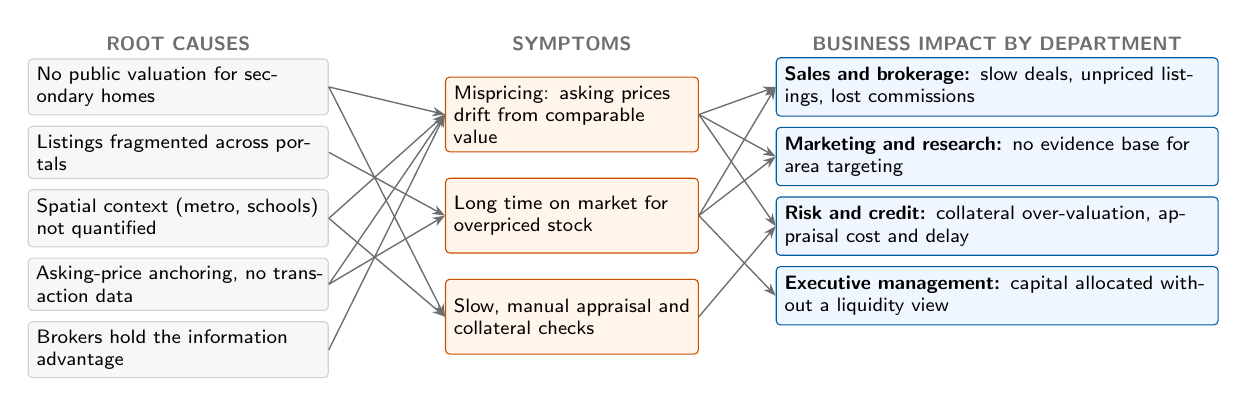
\begin{tikzpicture}[
  font=\sffamily\scriptsize,
  rc/.style={rounded corners=1.5pt, fill=lightgray, draw=rulecolor, text width=3.6cm, minimum height=0.62cm, align=left, inner sep=3pt},
  sy/.style={rounded corners=1.5pt, fill=orange!8!white, draw=accent, text width=3.0cm, minimum height=0.95cm, align=left, inner sep=3pt},
  im/.style={rounded corners=1.5pt, fill=metricbg, draw=brand, text width=5.4cm, minimum height=0.74cm, align=left, inner sep=3pt},
  hd/.style={font=\sffamily\bfseries\scriptsize, text=medgray},
  arr/.style={-{Stealth[length=1.6mm]}, color=medgray, line width=0.5pt}]
% root causes
\node[hd] at (0,0.55) {ROOT CAUSES};
\node[rc] (r1) at (0,0) {No public valuation for secondary homes};
\node[rc, below=0.13cm of r1] (r2) {Listings fragmented across portals};
\node[rc, below=0.13cm of r2] (r3) {Spatial context (metro, schools) not quantified};
\node[rc, below=0.13cm of r3] (r4) {Asking-price anchoring, no transaction data};
\node[rc, below=0.13cm of r4] (r5) {Brokers hold the information advantage};
% symptoms
\node[hd] at (5.0,0.55) {SYMPTOMS};
\node[sy] (s1) at (5.0,-0.35) {Mispricing: asking prices drift from comparable value};
\node[sy, below=0.32cm of s1] (s2) {Long time on market for overpriced stock};
\node[sy, below=0.32cm of s2] (s3) {Slow, manual appraisal and collateral checks};
% impact
\node[hd] at (10.4,0.55) {BUSINESS IMPACT BY DEPARTMENT};
\node[im] (i1) at (10.4,0) {\textbf{Sales and brokerage:} slow deals, unpriced listings, lost commissions};
\node[im, below=0.13cm of i1] (i2) {\textbf{Marketing and research:} no evidence base for area targeting};
\node[im, below=0.13cm of i2] (i3) {\textbf{Risk and credit:} collateral over-valuation, appraisal cost and delay};
\node[im, below=0.13cm of i3] (i4) {\textbf{Executive management:} capital allocated without a liquidity view};
\foreach \r in {r1,r4,r5} \draw[arr] (\r.east) -- (s1.west);
\foreach \r in {r2,r4} \draw[arr] (\r.east) -- (s2.west);
\foreach \r in {r1,r3} \draw[arr] (\r.east) -- (s3.west);
\draw[arr] (r3.east) -- (s1.west);
\draw[arr] (s1.east) -- (i1.west); \draw[arr] (s1.east) -- (i3.west);
\draw[arr] (s2.east) -- (i1.west); \draw[arr] (s2.east) -- (i4.west);
\draw[arr] (s3.east) -- (i3.west); \draw[arr] (s1.east) -- (i2.west); \draw[arr] (s2.east) -- (i2.west);
\end{tikzpicture} }
\exsource{team analysis; desk research in Section~\ref{sec:market}.}
\end{figure*}

\begin{table*}[t]
\caption{Existing tools serve project apartments or banks; no public tool values townhouses, villas and land in the secondary market}
\label{tab:competitors}
\tabsize
\begin{tabularx}{\textwidth}{@{}>{\bfseries}p{2.1cm}p{2.3cm}>{\hsize=1.35\hsize}Xp{2.5cm}p{2.1cm}>{\hsize=0.65\hsize}X@{}}
\toprule
Solution & Serves & Coverage (as reported) & Method & Access & Gap this platform addresses \\
\midrule
OneHousing (One Mount) & Buyers of project homes; Techcombank borrowers & 533,856 homes in 627 projects one month after the 2022 launch, mostly high-rise apartments \citep{onehousing_bpl2022}; company-reported error below 5\% \citep{onehousing_vne2022} & Proprietary model on developer and transaction data & Free lookup; paid valuation note accepted by Techcombank \citep{techcombank_avm} & Listed projects only; no alley houses, no land, no published method \\
Citics Valuation & Banks & Used by more than 32 banks; over 33 million properties digitised in 38 provinces; USD 2.1 million raised in 2025 \citep{citics_e27_2025} & Automated valuation inside the bank workflow & Institutions only & No buyer or broker access \\
Rever & Buyers and sellers via brokers & Brokerage with a technology layer \citep{rever2021} & Broker comparables & Through agents & No public valuation \\
Propzy & Brokerage platform & Closed in September 2022 after failing to raise capital \citep{propzy2022} & Broker comparables & Closed & Shows the cost of a capital-heavy model \\
Bank appraisal & Lenders & Every mortgage file & Site visit and comparables & Internal & Slow and costly per file \\
Broker judgement & Most secondary deals & All types & Personal comparables & Informal & No error band, no audit trail \\
\bottomrule
\end{tabularx}
\exsource{company pages and press reports cited in the table (figures as reported by the companies, not independently verified); team analysis.}
\end{table*}

\begin{problembox}
Buyers, independent brokers and lenders in Hanoi and Ho Chi Minh City set and accept prices for secondary-market homes without an independent reference. Existing valuation products cover listed apartment projects or serve banks only. Most townhouse, villa and land deals are therefore priced by anchoring on the asking price. The platform answers three questions: what is this home worth, is the asking price out of line, and which districts move slowly?
\end{problembox}

The same missing number, a fair value with a stated error, serves four groups that make different decisions (Exhibit~\ref{tab:stakeholders}). This makes the problem cross-functional: one tool, four uses.

\begin{table}[!b]
\caption{Each stakeholder needs the same fair-value reference for a different decision}
\label{tab:stakeholders}
\tabsize
\begin{tabularx}{\columnwidth}{@{}>{\bfseries}p{1.75cm}X X@{}}
\toprule
Stakeholder & Decision & What is missing today \\
\midrule
Buyers & Offer price, walk away or negotiate & No reference outside the listing itself \\
Brokers (sales) & List price advice, which sellers to coach & Comparables found by hand, no error band \\
Banks (risk, credit) & Loan amount at 70\% loan-to-value & Manual appraisal, slow and costly \\
Research, marketing & Which districts to target, with what message & No district view of price and speed \\
Executives & Where to open offices and commit capital & No combined price and speed map \\
\bottomrule
\end{tabularx}
\exsource{team analysis.}
\end{table}

\textbf{Two links carry most of the cost (Exhibit~\ref{fig:rootcause}).} First, without a public valuation, asking prices anchor negotiations and drift from the value of comparable homes. Brokers then lose time on listings that do not sell, and banks risk over-valuing collateral. Second, experienced brokers see the value of a metro station, a school or a short commute, but buyers cannot measure it. That gap preserves the broker's information advantage and slows every deal. Section~\ref{sec:xf} returns to the same four departments with evidence from the platform. 
% ---- inlined from sections/02_market ----
\section{Market scan and evidence base}
\label{sec:market}

\begin{table*}[t]
\caption{Research and practice shape every design choice: a transparent baseline, measured location, a stronger model and accuracy reported the way lenders read it}
\label{tab:evidence}
\tabsize
\begin{tabularx}{\textwidth}{@{}>{\bfseries}p{3.0cm}XX@{}}
\toprule
Question & What research and practice say & Design choice \\
\midrule
What drives housing prices? & A home is a bundle of attributes with implicit prices \citep{rosen1974}. Floor area, rooms, age and location recur across studies with consistent signs \citep{sirmans2005}. A log-price model with location effects is the standard starting point \citep{malpezzi2003}. & A transparent regression on log asking price with district effects is the baseline of the Fair Value Engine. \\
Does transport access raise prices? & Shorter distance to a new London rail station was associated with higher prices \citep{gibbons2005}; station effects vary widely across cities \citep{debrezion2007}. Hanoi runs two urban rail lines; HCMC Line 1 opened on 22 December 2024 \citep{hcmcmetro2024}. & Distance to the nearest operating station enters the engine. Its association with price is measured, not assumed. \\
Do machine-learning models beat regression? & On 123,000 Swiss sales, gradient boosting gave the most accurate valuations of six methods \citep{mayer2019}. XGBoost is a fast, regularised version \citep{chen2016}; SHAP values explain each estimate \citep{lundberg2017}. & Gradient boosting competes with the regression on the same unseen homes; SHAP charts explain it to managers. \\
How do practitioners judge accuracy? & The IAAO standards ask for testing on held-out sales, hit rates within a tolerance and ratio statistics \citep{iaao2018,iaao2013}. Prediction intervals with a coverage guarantee are available without distribution assumptions \citep{lei2018}. & Accuracy is reported as the share of estimates within ±10\% and ±20\% (PPE10, PPE20), with a 90\% range, by property type. \\
\bottomrule
\end{tabularx}
\exsource{studies, standards and company sources cited in the table; team analysis.}
\end{table*}

\textbf{The public, all-type quadrant is empty.} OneHousing is public but covers listed apartment projects. Citics covers all types but serves banks only (Exhibits~\ref{tab:competitors} and~\ref{fig:positioning}). Rever and Propzy built brokerages, not valuation tools, and Propzy closed in 2022. A buyer or broker pricing an alley house, a villa or a plot of land has no independent number to check.

\begin{figure}[!t]
\caption{No public tool values every property type}
\label{fig:positioning}
\centering
\resizebox{0.85\columnwidth}{!}{% ---- inlined from diagrams/positioning.tex ----
% Competitive positioning: x = property coverage, y = access (institutional -> public)
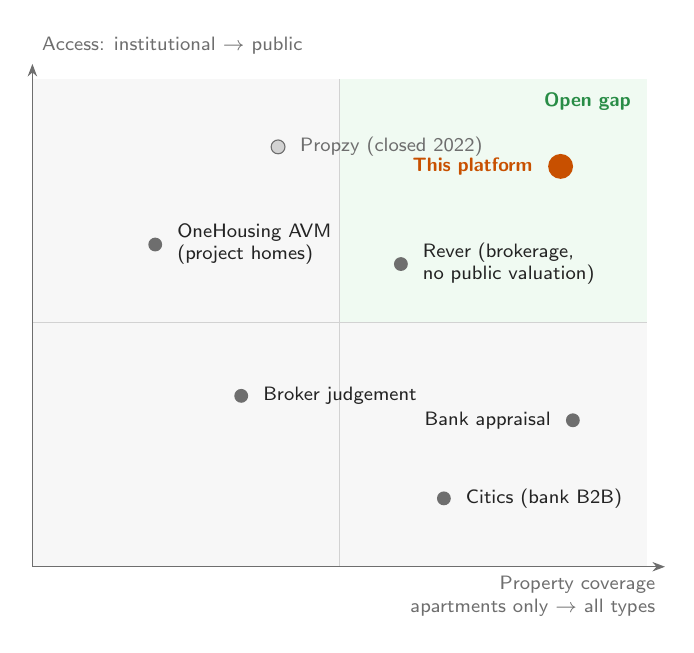
\begin{tikzpicture}[font=\sffamily\scriptsize, x=0.78cm, y=0.62cm,
  pl/.style={circle, inner sep=0pt, minimum size=5pt},
  lb/.style={font=\sffamily\scriptsize, text=darkgray, align=left}]
\fill[lightgray] (0,0) rectangle (10,10);
\fill[greenbg] (5,5) rectangle (10,10);
\draw[rulecolor] (5,0) -- (5,10); \draw[rulecolor] (0,5) -- (10,5);
\draw[-{Stealth[length=1.6mm]}, medgray] (0,0) -- (10.3,0) node[below left, text=medgray, align=right] {Property coverage\\apartments only $\rightarrow$ all types};
\draw[-{Stealth[length=1.6mm]}, medgray] (0,0) -- (0,10.3) node[above right, text=medgray] {Access: institutional $\rightarrow$ public};
\node[text=greenframe, font=\sffamily\bfseries\scriptsize, anchor=north east] at (9.9,9.9) {Open gap};
\node[pl, fill=medgray] at (2.0,6.6) {}; \node[lb, anchor=west] at (2.2,6.6) {OneHousing AVM\\(project homes)};
\node[pl, fill=medgray] at (6.7,1.4) {}; \node[lb, anchor=west] at (6.9,1.4) {Citics (bank B2B)};
\node[pl, fill=medgray] at (8.8,3.0) {}; \node[lb, anchor=east] at (8.6,3.0) {Bank appraisal};
\node[pl, fill=medgray] at (6.0,6.2) {}; \node[lb, anchor=west] at (6.2,6.2) {Rever (brokerage,\\no public valuation)};
\node[pl, fill=rulecolor, draw=medgray] at (4.0,8.6) {}; \node[lb, anchor=west, text=medgray] at (4.2,8.6) {Propzy (closed 2022)};
\node[pl, fill=medgray] at (3.4,3.5) {}; \node[lb, anchor=west] at (3.6,3.5) {Broker judgement};
\node[pl, fill=accent, minimum size=9pt] at (8.6,8.2) {}; \node[lb, anchor=east, font=\sffamily\bfseries\scriptsize, text=accent] at (8.3,8.2) {This platform};
\end{tikzpicture} }
\exsource{desk research (Exhibit~\ref{tab:competitors}); positions are team judgements.}
\end{figure}

\begin{valuebox}
\textbf{Where this platform differs.} It values all property types, including alley houses and land. It publishes its method and its error for each type. It adds measured location data from OpenStreetMap to the listings. It also ranks listings by the risk of staying unsold and maps the districts for managers.
\end{valuebox}

\textbf{Research and practice settle four design questions (Exhibit~\ref{tab:evidence}).} Academic studies explain what drives prices and which methods value homes best. Practice adds two lessons. Zillow publishes its error by market segment, and the off-market error is several times the on-market error \citep{zillow_zestimate}. Zillow also closed its home-buying arm in 2021 after its management said that forecasting home prices was harder than expected \citep{inman2021}. A valuation is a reference for a human decision, not an automatic bid. 
% ---- inlined from sections/04_data ----
\section{Data: two sources, one property table}
\label{sec:data}

\begin{figure*}[t]
\caption{Listings and map data are cleaned, matched by location and stored as one property table that serves all three engines}
\label{fig:architecture}
\centering
\resizebox{\textwidth}{!}{% ---- inlined from diagrams/architecture.tex ----
% Data architecture: sources -> raw store -> cleaning and location matching -> integrated table -> engines -> outputs
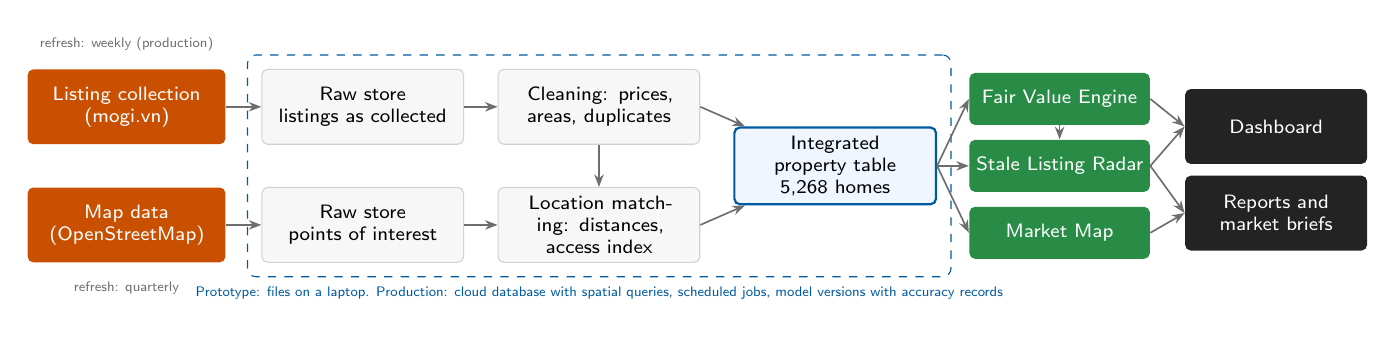
\begin{tikzpicture}[
  font=\sffamily\scriptsize,
  src/.style={rounded corners=2pt, fill=accent, text=white, text width=2.3cm, align=center, minimum height=0.95cm, inner sep=3pt},
  lay/.style={rounded corners=2pt, fill=lightgray, draw=rulecolor, text width=2.35cm, align=center, minimum height=0.95cm, inner sep=3pt},
  mod/.style={rounded corners=2pt, fill=greenframe, text=white, text width=2.15cm, align=center, minimum height=0.66cm, inner sep=2pt},
  outb/.style={rounded corners=2pt, fill=darkgray, text=white, text width=2.1cm, align=center, minimum height=0.95cm, inner sep=3pt},
  note/.style={font=\sffamily\tiny, text=medgray, align=center},
  arr/.style={-{Stealth[length=1.6mm]}, color=medgray, line width=0.6pt}]
\node[src] (m) at (0,0.75) {Listing collection\\(mogi.vn)};
\node[src] (o) at (0,-0.75) {Map data\\(OpenStreetMap)};
\node[lay] (raw) at (3.0,0.75) {Raw store\\listings as collected};
\node[lay] (cache) at (3.0,-0.75) {Raw store\\points of interest};
\node[lay] (cl) at (6.0,0.75) {Cleaning: prices, areas, duplicates};
\node[lay] (sj) at (6.0,-0.75) {Location matching: distances, access index};
\node[lay, fill=metricbg, draw=brand, line width=0.8pt] (tab) at (9.0,0) {Integrated property table\\ \Nclean{} homes};
\node[mod] (m1) at (11.85,0.85) {Fair Value Engine};
\node[mod] (m2) at (11.85,0) {Stale Listing Radar};
\node[mod] (m3) at (11.85,-0.85) {Market Map};
\node[outb] (dash) at (14.6,0.5) {Dashboard};
\node[outb] (rep) at (14.6,-0.6) {Reports and market briefs};
\draw[arr] (m) -- (raw); \draw[arr] (o) -- (cache); \draw[arr] (raw) -- (cl); \draw[arr] (cache) -- (sj);
\draw[arr] (cl) -- (sj); \draw[arr] (cl.east) -- (tab); \draw[arr] (sj.east) -- (tab);
\draw[arr] (tab.east) -- (m1.west); \draw[arr] (tab.east) -- (m2.west); \draw[arr] (tab.east) -- (m3.west);
\draw[arr] (m1) -- (m2);
\draw[arr] (m1.east) -- (dash.west); \draw[arr] (m2.east) -- (dash.west); \draw[arr] (m3.east) -- (rep.west); \draw[arr] (m2.east) -- (rep.west);
\node[note] at (0,1.55) {refresh: weekly (production)};
\node[note] at (0,-1.55) {refresh: quarterly};
\begin{scope}[on background layer]
\node[fit=(raw)(cache)(cl)(sj)(tab), draw=brand, dashed, rounded corners=3pt, inner sep=5pt] (prod) {};
\end{scope}
\node[note, text=brand, anchor=north] at (prod.south) {Prototype: files on a laptop. Production: cloud database with spatial queries, scheduled jobs, model versions with accuracy records};
\end{tikzpicture} }
\exsource{team design.}
\end{figure*}

\begin{table*}[t]
\caption{Example extract: eight clean listings across both cities and four property types}
\label{tab:sample}
\centering
\resizebox{\textwidth}{!}{% ---- inlined from tables/sample_extract.tex ----
\begin{tabular}{rlllrrrrll}
\toprule
ID & City & District (as listed) & Type (site label) & Price (VND bn) & Area (m$^2$) & VND m/m$^2$ & Beds & Legal & Posted \\
\midrule
21710182 & TP. Hồ Chí Minh & Quận 10 & Căn hộ chung cư & 3.50 & 50 & 70.0 & 1 & Khác & 14/10/2026 \\
22751445 & TP. Hồ Chí Minh & Quận Gò Vấp & Nhà hẻm/ngõ & 4.25 & 40 & 106.2 & 3 & Sổ hồng & 09/10/2026 \\
22715805 & TP. Hồ Chí Minh & Quận 1 & Nhà mặt tiền/phố & 35.00 & 71 & 493.0 & 13 & Sổ hồng & 15/10/2026 \\
22726003 & TP. Hồ Chí Minh & Quận 12 & Đất & 5.19 & 92 & 56.4 & 0 & Sổ hồng & 12/10/2026 \\
22673730 & Hà Nội & Quận Cầu Giấy & Căn hộ chung cư & 9.72 & 136 & 71.5 & 3 & Sổ đỏ & 18/04/2025 \\
22747097 & Hà Nội & Quận Đống Đa & Nhà hẻm/ngõ & 12.50 & 50 & 250.0 & 6 & Sổ đỏ & 16/08/2026 \\
22415247 & Hà Nội & Quận Đống Đa & Nhà mặt tiền/phố & 49.90 & 131 & 380.9 & 8 & Sổ đỏ & 14/08/2026 \\
22723649 & Hà Nội & Quận Tây Hồ & Đất & 31.80 & 151 & 210.6 & 0 & Sổ đỏ & 31/12/2025 \\
\bottomrule
\end{tabular} }
\exsource{\srcmogi; prices are asking prices; VND m/m$^2$ = million VND per square metre.}
\end{table*}

\textbf{One property table feeds all three engines (Exhibit~\ref{fig:architecture}).} Listings from mogi.vn supply prices and home attributes. OpenStreetMap supplies the location context: metro stations, schools, hospitals, parks, markets and water. Both are cleaned, matched by map position and stored as one table.

\textbf{The sample is a prototype sized for a 1.5-hour collection window.} The collector gathered \Nraw{} sale listings with their detail pages in \scrapeMinutes{} minutes on \scrapeDate{}: \throughput{} listings an hour, with no blocked requests. Quotas per city were set by type, so type shares reflect the quotas, not the market (Exhibit~\ref{tab:sources}). Hanoi apartments ran out after about \supplyAptHN{} listings, and the shortfall moved to other types. The site lists newest first, so a fifth of each quota came from the last result pages to include older listings. A scheduled run covers the full market of at least \supplyTotal{} listings in about \fullRunHours{} hours.

\begin{table}[!t]
\caption{Listings supply prices and attributes; map data supplies location; every type has enough homes to report accuracy}
\label{tab:sources}
\tabsize
\begin{tabularx}{\columnwidth}{@{}>{\bfseries}p{1.5cm}XX@{}}
\toprule
 & mogi.vn listings & OpenStreetMap \\
\midrule
Content & Asking price, area, rooms, legal status, address, map point, text & \NpoiTotal{} points: \NmetroHN{} + \NmetroHCM{} metro stations, \NbusStops{} bus stops, schools, hospitals, parks, markets, water \\
Refresh & Weekly in production & Quarterly \\
Licence & Public pages, research use & Open Database Licence \\
Sample & \Nraw{} collected, \Nclean{} clean: \NcleanHN{} Hanoi, \NcleanHCM{} HCMC; \Ndistricts{} districts & 9 layers, 2 cities \\
\midrule
\multicolumn{3}{@{}l}{\textbf{Clean homes by type:} apartments \NtypeApartment, alley houses \NtypeAlleyHouse,} \\
\multicolumn{3}{@{}l}{street-front houses \NtypeStreetFrontHouse, villas and terraced \NtypeVillaTerraced, land \NtypeLand} \\
\bottomrule
\end{tabularx}
\exsource{\srcmogi; \srcosm.}
\end{table}

\textbf{Each home carries four groups of facts (Exhibit~\ref{tab:sample}).} Physical facts: area, rooms, storeys, frontage and access road width. Legal status. Text flags from the description, such as car access, corner lot or business use. Location: distances to the centre and to the nearest metro station, school, hospital, park and market, plus one accessibility score. Missing values are filled with the typical value for the type and flagged, so the engines can learn whether a gap itself carries information.

\textbf{Cleaning kept \cleanShare{} of the listings (Exhibit~\ref{fig:waterfall}).} The largest loss is the same home posted by several brokers (\dropDup). Areas out of range (\dropArea), buildings with more than 15 bedrooms sold as serviced apartments (\dropBeds) and placeholder or mistyped prices (\dropImplausible) follow. The price reader matches the site's own numeric price on \priceAgree{} of listings.

\begin{figure}[!t]
\caption{\cleanShare{} of collected listings survive cleaning; duplicate postings remove the most}
\label{fig:waterfall}
\centering
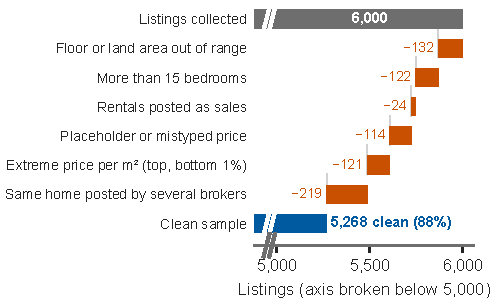
\includegraphics[width=\columnwidth]{cleaning_waterfall.pdf}
\exsource{\srcmogi; team analysis.}
\end{figure}

\subsection{Integration challenges}
\begin{itemize}
\item \textbf{Location precision.} \sharePoint{} of listings carry the poster's own map pin; \shareWardCentroid{} share a pin with listings on other streets, so their distances are accurate to the ward, not the plot.
\item \textbf{Administrative reform.} Since 1 July 2025 Vietnam has no districts and many wards were merged \citep{pwc2025}. The site still uses the old names, so the platform does too.
\item \textbf{Asking, not transaction, prices.} The engine estimates what comparable sellers ask. Calibration on transaction prices is part of the roadmap (Section~\ref{sec:roadmap}).
\item \textbf{Refreshed dates.} Sellers re-post listings, which resets the posted date. Listing age is therefore measured from the creation date implied by the listing ID.
\end{itemize}

\subsection{Privacy and ethics}
\begin{itemize}
\item Only public listing pages were collected, on paths that the site's robots.txt allows; requests were paced and identified as research.
\item Phone numbers and e-mail addresses were removed before saving; no agent names or profile links were stored.
\item OpenStreetMap data is used under the Open Database Licence with attribution.
\end{itemize} 
% ---- inlined from sections/05_design ----
\section{How the platform works}
\label{sec:design}

\begin{figure*}[t]
\caption{Three linked engines turn one property table into three decisions: price and lend, coach and prioritise, target and allocate}
\label{fig:pipeline}
\centering
\resizebox{0.86\textwidth}{!}{% ---- inlined from diagrams/pipeline.tex ----
% Analytical pipeline: how the three engines connect and which decision each feeds
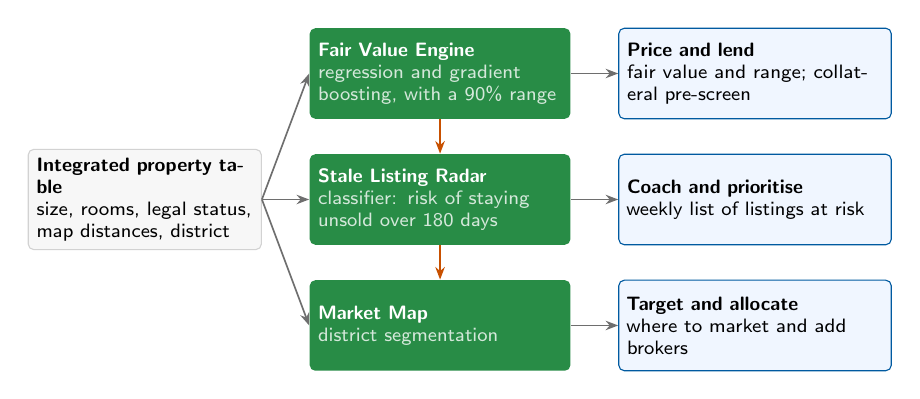
\begin{tikzpicture}[
  font=\sffamily\scriptsize,
  st/.style={rounded corners=2pt, fill=lightgray, draw=rulecolor, text width=2.75cm, align=left, minimum height=1.15cm, inner sep=3pt},
  md/.style={rounded corners=2pt, fill=greenframe, text=white, text width=3.1cm, align=left, minimum height=1.15cm, inner sep=3pt},
  dc/.style={rounded corners=2pt, fill=metricbg, draw=brand, text width=3.25cm, align=left, minimum height=1.15cm, inner sep=3pt},
  arr/.style={-{Stealth[length=1.6mm]}, color=medgray, line width=0.6pt}]
\node[st] (in) at (0,0) {\textbf{Integrated property table}\\size, rooms, legal status, map distances, district};
\node[md] (m1) at (3.75,1.6) {\textbf{Fair Value Engine}\\{\color{white!80!greenframe}regression and gradient boosting, with a 90\% range}};
\node[md] (m2) at (3.75,0) {\textbf{Stale Listing Radar}\\{\color{white!80!greenframe}classifier: risk of staying unsold over \staleDays{} days}};
\node[md] (m3) at (3.75,-1.6) {\textbf{Market Map}\\{\color{white!80!greenframe}district segmentation}};
\node[dc] (d1) at (7.75,1.6) {\textbf{Price and lend}\\fair value and range; collateral pre-screen};
\node[dc] (d2) at (7.75,0) {\textbf{Coach and prioritise}\\weekly list of listings at risk};
\node[dc] (d3) at (7.75,-1.6) {\textbf{Target and allocate}\\where to market and add brokers};
\draw[arr] (in.east) -- (m1.west); \draw[arr] (in.east) -- (m2.west); \draw[arr] (in.east) -- (m3.west);
\draw[arr, color=accent, line width=0.9pt] (m1.south) -- (m2.north);
\draw[arr, color=accent, line width=0.9pt] (m2.south) -- (m3.north);
\draw[arr] (m1) -- (d1); \draw[arr] (m2) -- (d2); \draw[arr] (m3) -- (d3);
\end{tikzpicture} }
\exsource{team design.}
\end{figure*}

\textbf{Three engines share one table, and each ends in a decision owned by a department (Exhibit~\ref{fig:pipeline}).} The \textbf{Fair Value Engine} combines a transparent hedonic regression with a gradient-boosting valuation model and shows a 90\% range around each estimate. The \textbf{Stale Listing Radar} is a classifier that ranks listings by the risk of staying unsold for more than \staleDays{} days. It uses the gap between the asking price and the fair value as one of its inputs. The \textbf{Market Map} groups districts by price, speed, access and housing mix.

\textbf{Each engine has an accuracy target for broker use.} The regression should explain more than 75\% of the variation in asking prices (R$^2$ above 0.75). The valuation model should reach a typical error below 0.20 on the log scale (RMSE). For lenders, the same error is restated as the share of estimates within ±10\% and ±20\% of the asking price (PPE10, PPE20). The radar should rank stale listings with an AUC above 0.72, where 0.5 is a coin flip and 1.0 a perfect ranking. The district segments should be distinct enough to target separately.

\subsection{How the results were kept honest}
Every accuracy figure comes from homes the engines had not seen while they were built. The radar never sees listing age, dates or anything that would reveal the answer. Listing age is measured from the creation date, because sellers refresh the posted date when they re-post (Appendix~\ref{app:safeguards}). 
% ---- inlined from sections/06_results ----
\section{Results}
\label{sec:results}

\begin{figure*}[t]
\caption{The gradient-boosting model beats the regression on every accuracy measure: \xgbPPEtwenty{} of estimates fall within ±20\% of the asking price}
\label{fig:avmperf}
\centering
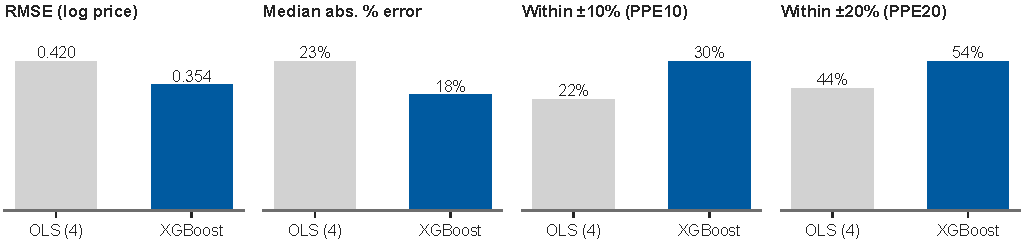
\includegraphics[width=\textwidth]{avm_performance.pdf}
\exsource{\srcmogi; \srcosm; \Ntest{} test homes not used to build the models, stratified by city and type; team analysis.}
\end{figure*}

\subsection{Fair Value Engine: what a home is worth}
\label{sec:m1}

\textbf{Location explains a quarter of valuation error, and map data captures most of it without knowing the district.} Size, rooms and legal status alone explain \RtwoA{} of the variation in asking prices. Adding the district cuts the valuation error by \cutDistrict{}. Measured distances to the centre, metro, schools and markets, without the district, cut it by \cutOSMnoFE{}, about \shareOSMofFE{} of the district gain (Exhibit~\ref{tab:ladder}). For the business this means the engine can value homes in districts with few listings, where comparables are hardest to find.

\begin{table}[!t]
\caption{Map data alone recovers \shareOSMofFE{} of the accuracy gain from knowing the district}
\label{tab:ladder}
\tabsize
\begin{tabularx}{\columnwidth}{@{}Xrrr@{}}
\toprule
Information used & R$^2$ & Typical error & Error cut \\
\midrule
Size, rooms, legal status & \RtwoA & \cvA & base \\
+ district & \RtwoB & \cvB & \cutDistrict \\
+ map distances, no district & \RtwoE & \cvE & \cutOSMnoFE \\
+ district and map distances & \RtwoC & \cvC & \cutOSMfromPhys \\
+ type-specific size effects & \RtwoD & \cvD & \cutTotal \\
\bottomrule
\end{tabularx}
\exsource{\srcmogi; \srcosm; regression on log asking price; typical error = cross-validated RMSE on the log scale; full table in Appendix~\ref{app:ladder}.}
\end{table}

\textbf{Distance to the centre costs more in Hanoi than in HCMC.} Before any adjustment, a home twice as far from the centre asks about \twiceFarHN{} less per m$^2$ in Hanoi and \twiceFarHCM{} less in HCMC. Property type matters as much as place. Street-front houses ask \ratioSFaptHN{} to \ratioSFaptHCM{} times the apartment price per m$^2$, because their price is quoted per m$^2$ of land and includes business value. Accuracy must therefore be judged type by type, never as one average.

\textbf{Size, height, road access and title drive the price.} A 10\% larger home asks about \areaTen{} more. Each extra storey is associated with \pctStoreys{} higher asking prices and each metre of access road width with \pctRoad{}, holding district and amenities constant. Listings with an unknown or informal legal status ask about \pctOtherLegalAbs{} less than those with a red or pink book. These are associations in asking prices, not causal effects.

\textbf{The gradient-boosting model is the better engine (Exhibit~\ref{fig:avmperf}).} On \Ntest{} homes it had not seen, it places \xgbPPEtwenty{} of estimates within ±20\% of the asking price, against \olsPPEtwenty{} for the regression. The regression meets its target (R$^2$ \RtwoD{} against 0.75). The typical error of the boosting model, \xgbRMSE{} on the log scale, misses the 0.20 target. Half of all estimates miss by more than \xgbMdAPE, so the engine needs a range, not a single number.

\textbf{Accuracy differs by type, and that sets the launch scope.} \ppeTwentyAlleyHouse{} of alley houses and \ppeTwentyApartment{} of apartments fall within ±20\%. Villas reach \ppeTwentyVillaTerraced, land \ppeTwentyLand{} and street-front houses \ppeTwentyStreetFrontHouse; listing fields capture poorly what makes a frontage valuable. The 90\% range covers \confCovType{} of test homes as intended. It spans \confWidthAlleyHouse{} of the estimate for alley houses but \confWidthLand{} for land. Expensive homes tend to be under-valued relative to cheap ones, which lenders must monitor (Appendix~\ref{app:metrics}).

\begin{figure}[!t]
\caption{Size and building attributes set the level; distance to the centre and to metro are the strongest location drivers}
\label{fig:avmshap}
\centering
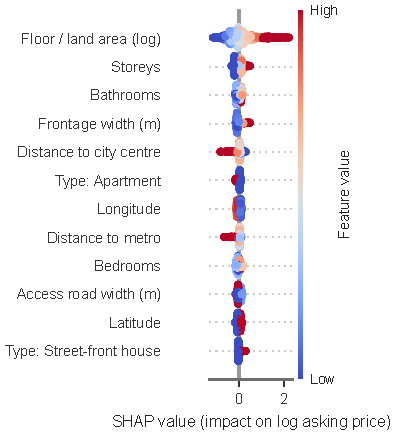
\includegraphics[width=\columnwidth]{avm_shap_summary.pdf}
\exsource{\srcmogi; \srcosm; contribution of each input to the test-set estimates (SHAP values), top 12 inputs excluding district.}
\end{figure}

\textbf{Area dominates the estimate, then \avmTopTwo{} and \avmTopThree{} (Exhibit~\ref{fig:avmshap}).} Distance to the centre and to the nearest metro station are the strongest location drivers. The value is flat across the inner districts and falls beyond them. With only \NmetroHN{} stations in Hanoi and \NmetroHCM{} in HCMC, metro distance mostly separates the core from the periphery. A premium for homes next to a station cannot yet be isolated.

\begin{insightbox}
Launch the engine as a pricing reference for apartments and alley houses, always with its range. Villas, land and street-front houses need a desk review until frontage and plot data improve.
\end{insightbox}

\begin{figure*}[t]
\caption{The Stale Listing Radar separates stale from fresh listings with an AUC of \xgbAUC; a rule based on the price gap does no better than a coin flip}
\label{fig:roc}
\centering
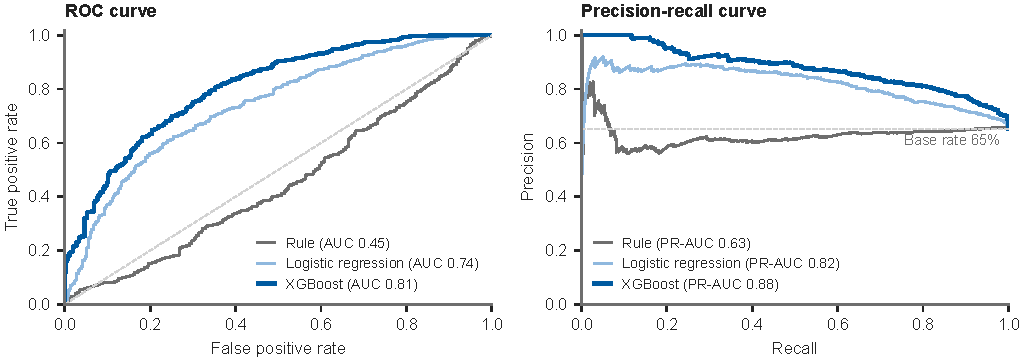
\includegraphics[width=\textwidth]{stale_roc_pr.pdf}
\exsource{\srcmogi; \NstaleTest{} test listings; team analysis.}
\end{figure*}

\begin{figure*}[t]
\caption{Listings in the top 10\% of risk scores are stale \topDecileLift{} times as often as the average listing; costlier misses push the alert threshold down}
\label{fig:gains}
\centering
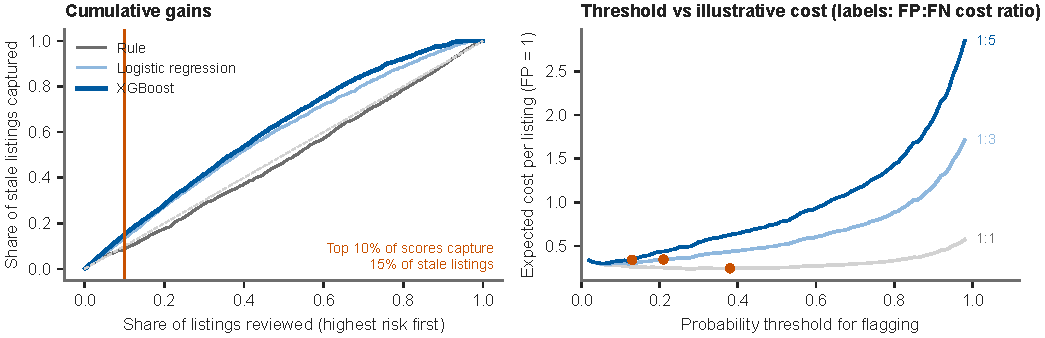
\includegraphics[width=\textwidth]{stale_gains_cost.pdf}
\exsource{\srcmogi; test listings; costs are illustrative team assumptions (a false alert costs 1 unit).}
\end{figure*}

\subsection{Stale Listing Radar: which listings will sit unsold}
\label{sec:m2}

\textbf{The radar ranks stale risk well enough to plan a weekly review list.} A listing counts as stale when it has been on the site for more than \staleDays{} days since creation. At 90 days, \staleShareNinety{} of listings would count as stale, too many to separate, so the main specification uses \staleDays{} days (\stalePosShare{} stale). Checks at 60, 90 and 120 days are in the appendix. The radar reaches an AUC of \xgbAUC{} (95\% interval \xgbAUClo{} to \xgbAUChi), against \logitAUC{} for a logistic regression (Exhibit~\ref{fig:roc}).

\textbf{The top of the list is where the value is (Exhibit~\ref{fig:gains}).} Listings in the top 10\% of scores are stale \topDecileLift{} times as often as the average listing: \topDecilePrecision{} against a base rate of \baseRate. Because most listings are stale, the operational flag covers the top quarter of scores, a review load of one listing in four. If a missed stale listing costs five times a false alert, the best threshold flags \costFlagFive{} of listings instead of \costFlagOne.

\textbf{The alert threshold is a business choice, not a model setting.} At the threshold that balances misses and false alerts on training data, the radar finds \staleRecall{} of stale test listings, and \stalePrecision{} of its alerts are correct. A sales manager with a small team should use the top-quarter list. A manager who loses more from a missed stale listing than from a wasted review should lower the threshold.

\begin{figure}[!t]
\caption{District speed and the seller's profile drive stale risk; the price gap ranks \residRank{} of \NstaleFeatures}
\label{fig:staleshap}
\centering
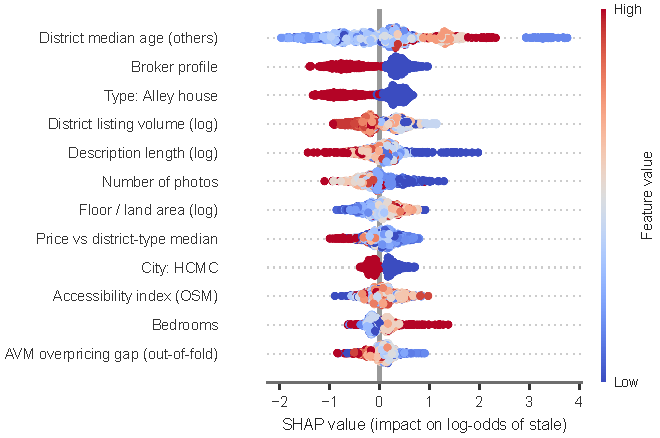
\includegraphics[width=\columnwidth]{stale_shap_summary.pdf}
\exsource{\srcmogi; contribution of each input to the test-set risk scores (SHAP values).}
\end{figure}

\textbf{Listings that sit unsold are not mainly overpriced listings.} A rule that flags listings asking more than 15\% above fair value scores an AUC of \ruleAUC, no better than a coin flip. The price gap ranks \residRank{} of \NstaleFeatures{} inputs (Exhibit~\ref{fig:staleshap}). The top drivers are how fast other listings in the district sell, whether a registered broker posted the listing, and the property type. Older listings even ask slightly less than their fair value. A plausible reason is that they were priced in an earlier, cheaper market and never repriced.

\begin{insightbox}
Use the radar to decide where brokers spend effort and the price gap to decide what to tell a seller. A true time-to-sale label from weekly data collection will sharpen both.
\end{insightbox}

\begin{figure*}[t]
\caption{Four district segments: a small prime core, two mid-market belts that differ by housing type and speed, and a land-led periphery}
\label{fig:segprofile}
\centering
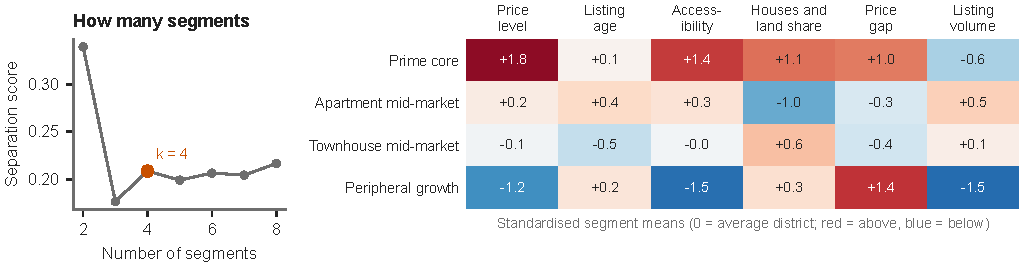
\includegraphics[width=\textwidth]{segments_profile.pdf}\\[4pt]
{\tabsize% ---- inlined from tables/segment_profiles.tex ----
\begin{tabular}{lrrrrrrr}
\toprule
Segment & Districts & Listings & Price/m$^2$ & Age & Access & Houses, land & To centre \\
 & (HN) & & (VND m) & (days) & index & share & (km) \\
\midrule
Prime core & 3 (1) & 249 & 415 & 328 & +1.41 & 84\% & 1.7 \\
Apartment mid-market & 13 (6) & 2,487 & 111 & 364 & +0.18 & 46\% & 6.1 \\
Townhouse mid-market & 14 (6) & 2,201 & 114 & 254 & -0.17 & 78\% & 7.3 \\
Peripheral growth & 4 (4) & 149 & 118 & 278 & -1.59 & 71\% & 13.6 \\
\bottomrule
\end{tabular} }
\exsource{\srcmogi; \srcosm; \NdistKept{} districts with at least 30 listings; table shows medians across the districts of each segment; team analysis.}
\end{figure*}

\begin{figure*}[t]
\caption{The prime core sits at the centre of each city; apartment and townhouse belts surround it, and the land-led periphery lies in Hanoi's outer districts}
\label{fig:segmaps}
\centering
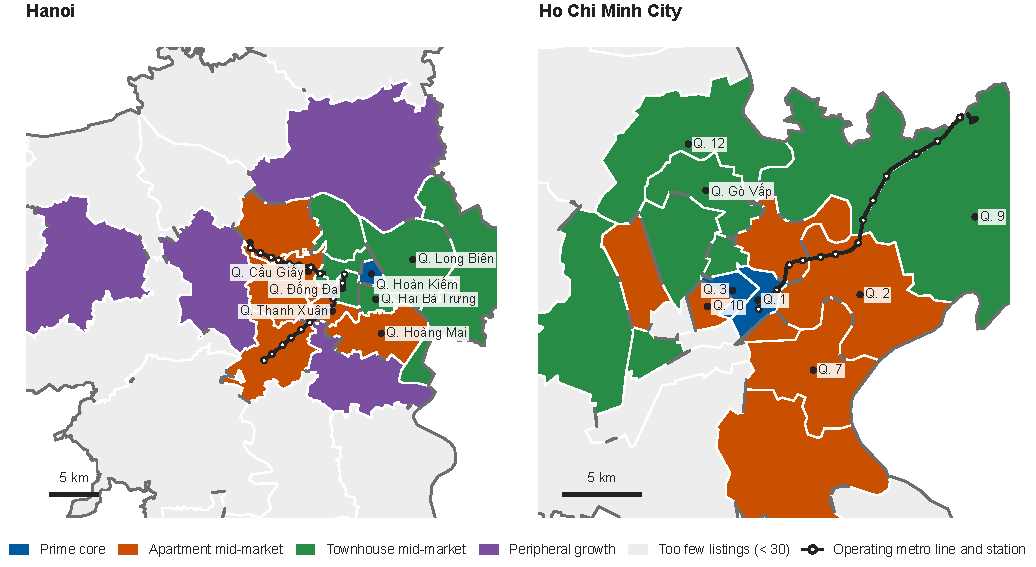
\includegraphics[width=\textwidth]{segments_maps.pdf}
\exsource{\srcmogi; \srcosm; district boundaries: GADM 4.1 (pre-2025 districts, as listed on the site); Nhà Bè (Apartment mid-market) lies south of the HCMC frame; team analysis.}
\end{figure*}

\subsection{Market Map: how districts differ}
\label{sec:m3}

\textbf{Four district segments give managers four different messages.} The map groups the \NdistKept{} districts with at least 30 listings (\segCover{} of listings) by price level, listing age, accessibility, housing mix, price gap and volume. The four segments overlap; treat them as targeting groups, not hard borders.
\begin{itemize}
\item \textbf{\segAname} (\segAdistricts) asks \segAppm{} million VND per m$^2$, \ratioPrime{} times the mid-market level, at a median \segAcbd{} km from the centre.
\item \textbf{\segBname} (\segBn{} districts, \segBlistings{} listings) is the slowest segment: median listing age \segBage{} days.
\item \textbf{\segCname} (\segCn{} districts) is house-heavy and the fastest (\segCage{} days), with the lowest stale-risk share (\segCrisk).
\item \textbf{\segDname} (\segDn{} Hanoi districts, \segDcbd{} km out) has the lowest access, the highest price gap and the highest stale-risk share (\segDrisk).
\end{itemize}
Exhibit~\ref{fig:segprofile} profiles the segments and Exhibit~\ref{fig:segmaps} shows where they sit. The two mid-market belts hold \segBlistings{} and \segClistings{} listings, most of the market, so they decide broker workload. The small prime core carries the highest prices and the small periphery the highest stale risk.

\begin{insightbox}
Defend price in the prime core, push slow apartment-belt listings harder, use the fast townhouse belt for volume and treat the periphery as a land market. Review segment borders each quarter.
\end{insightbox} 
% ---- inlined from sections/07_crossfunctional ----
\section{Impact by department}
\label{sec:xf}

\begin{figure*}[t]
\caption{Sales: stale risk concentrates in a few districts, and more than a third of street-front and land listings ask over 15\% above fair value}
\label{fig:xfsales}
\centering
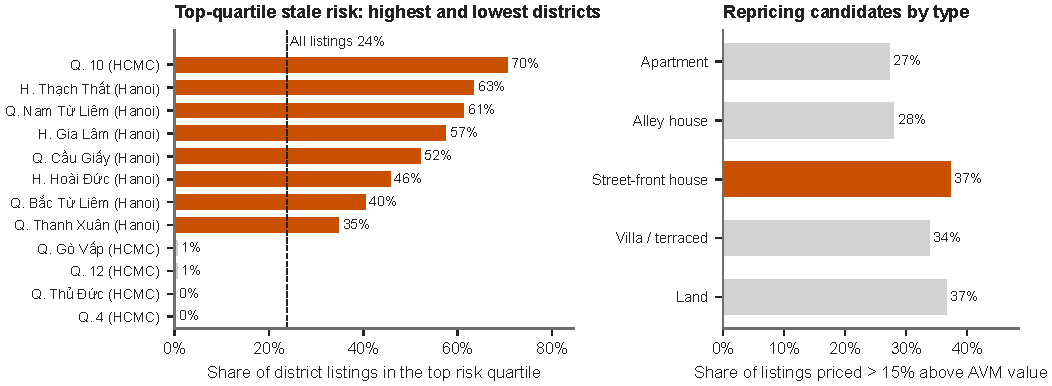
\includegraphics[width=\textwidth]{xf_sales.pdf}
\exsource{\srcmogi; fair values and risk scores estimated on listings the models had not seen; districts with at least 30 listings; team analysis.}
\end{figure*}

\textbf{The same three outputs serve four departments, each with its own decision and KPI.} The fair value with its range, the stale-risk rank and the district segment reach sales, marketing, risk and management in different forms.

\subsection{Sales and brokerage}
\textbf{Decision:} which sellers to coach on price and which listings to prioritise. \textbf{Evidence:} the share of listings in the top quarter of stale risk ranges from \topRiskShare{} in \topRiskDistrict{} to \lowRiskShare{} in \lowRiskDistrict{} (Exhibit~\ref{fig:xfsales}). Repricing candidates, listings asking more than 15\% above fair value, are most common for street-front houses (\overFifteenStreetFrontHouse) and land (\overFifteenLand), against \overFifteenApartment{} for apartments. \textbf{Talking point:} in high-risk districts, open the price conversation early with the range and comparables. \textbf{KPI:} median days to sale, coached against uncoached listings.

\subsection{Marketing and research}
\textbf{Decision:} which areas to target and with what message. \textbf{Evidence:} the four segments differ in price level, speed and housing mix (Exhibit~\ref{fig:segprofile}). \textbf{Messages:} scarcity and status in the \segAname{}; value and amenities in the slow \segBname{}, where listings need the most support. Speed and choice suit the \segCname{}; land and future infrastructure suit the \segDname{}. \textbf{KPI:} leads per listing by segment and campaign.

\begin{figure*}[t]
\caption{Risk: no property type is yet safe for collateral checks without a desk review; street-front houses and land carry the most over-valuation risk}
\label{fig:xfrisk}
\centering
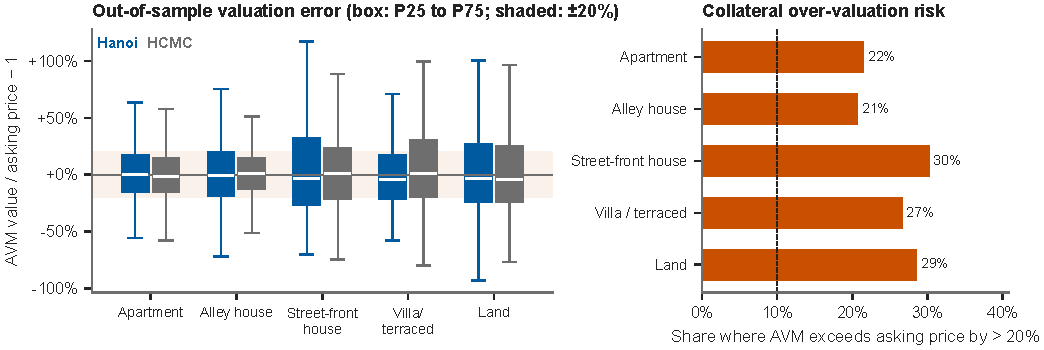
\includegraphics[width=\textwidth]{xf_risk.pdf}
\exsource{\srcmogi; fair values estimated on listings the models had not seen; team analysis.}
\end{figure*}

\subsection{Risk and credit}
\textbf{Decision:} when a fair value can pre-screen collateral before a manual appraisal. \textbf{Evidence:} the engine values \overAll{} of listings more than 20\% above their asking price (Exhibit~\ref{fig:xfrisk}). At a 70\% loan-to-value ratio such a case would lend 84\% of the asking price. Over-valuation is least frequent for alley houses (\overAlleyHouse) and apartments (\overApartment) and most frequent for street-front houses (\overStreetFrontHouse) and land (\overLand). \textbf{Rule:} fair value plus desk review for apartments, alley houses and villas; manual appraisal for street-front houses and land. \textbf{KPI:} share of pre-screens confirmed within ±10\% by the final appraisal.

\begin{figure*}[t]
\caption{Management: fast, high-priced districts sit in the upper left and deserve the most broker capacity}
\label{fig:execmatrix}
\centering
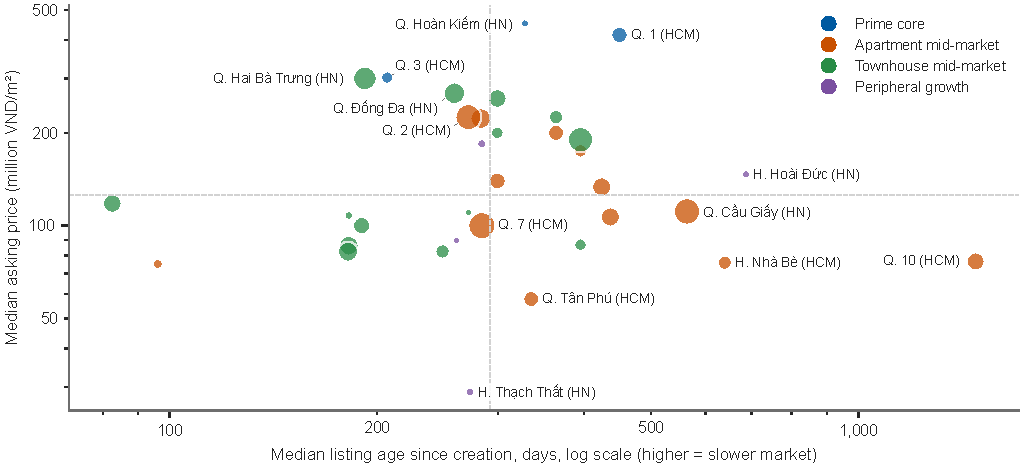
\includegraphics[width=0.74\textwidth]{executive_matrix.pdf}
\exsource{\srcmogi; \srcosm; bubble size = listings; dashed lines = medians across districts; team analysis.}
\end{figure*}

\begin{figure*}[t]
\caption{A broker enters a home and an asking price and reads the fair value, its range, the price gap, the stale-risk light, comparables and the district segment}
\label{fig:dashboard}
\centering
\begin{tikzpicture}
\node[anchor=south west, inner sep=0] (img) at (0,0) {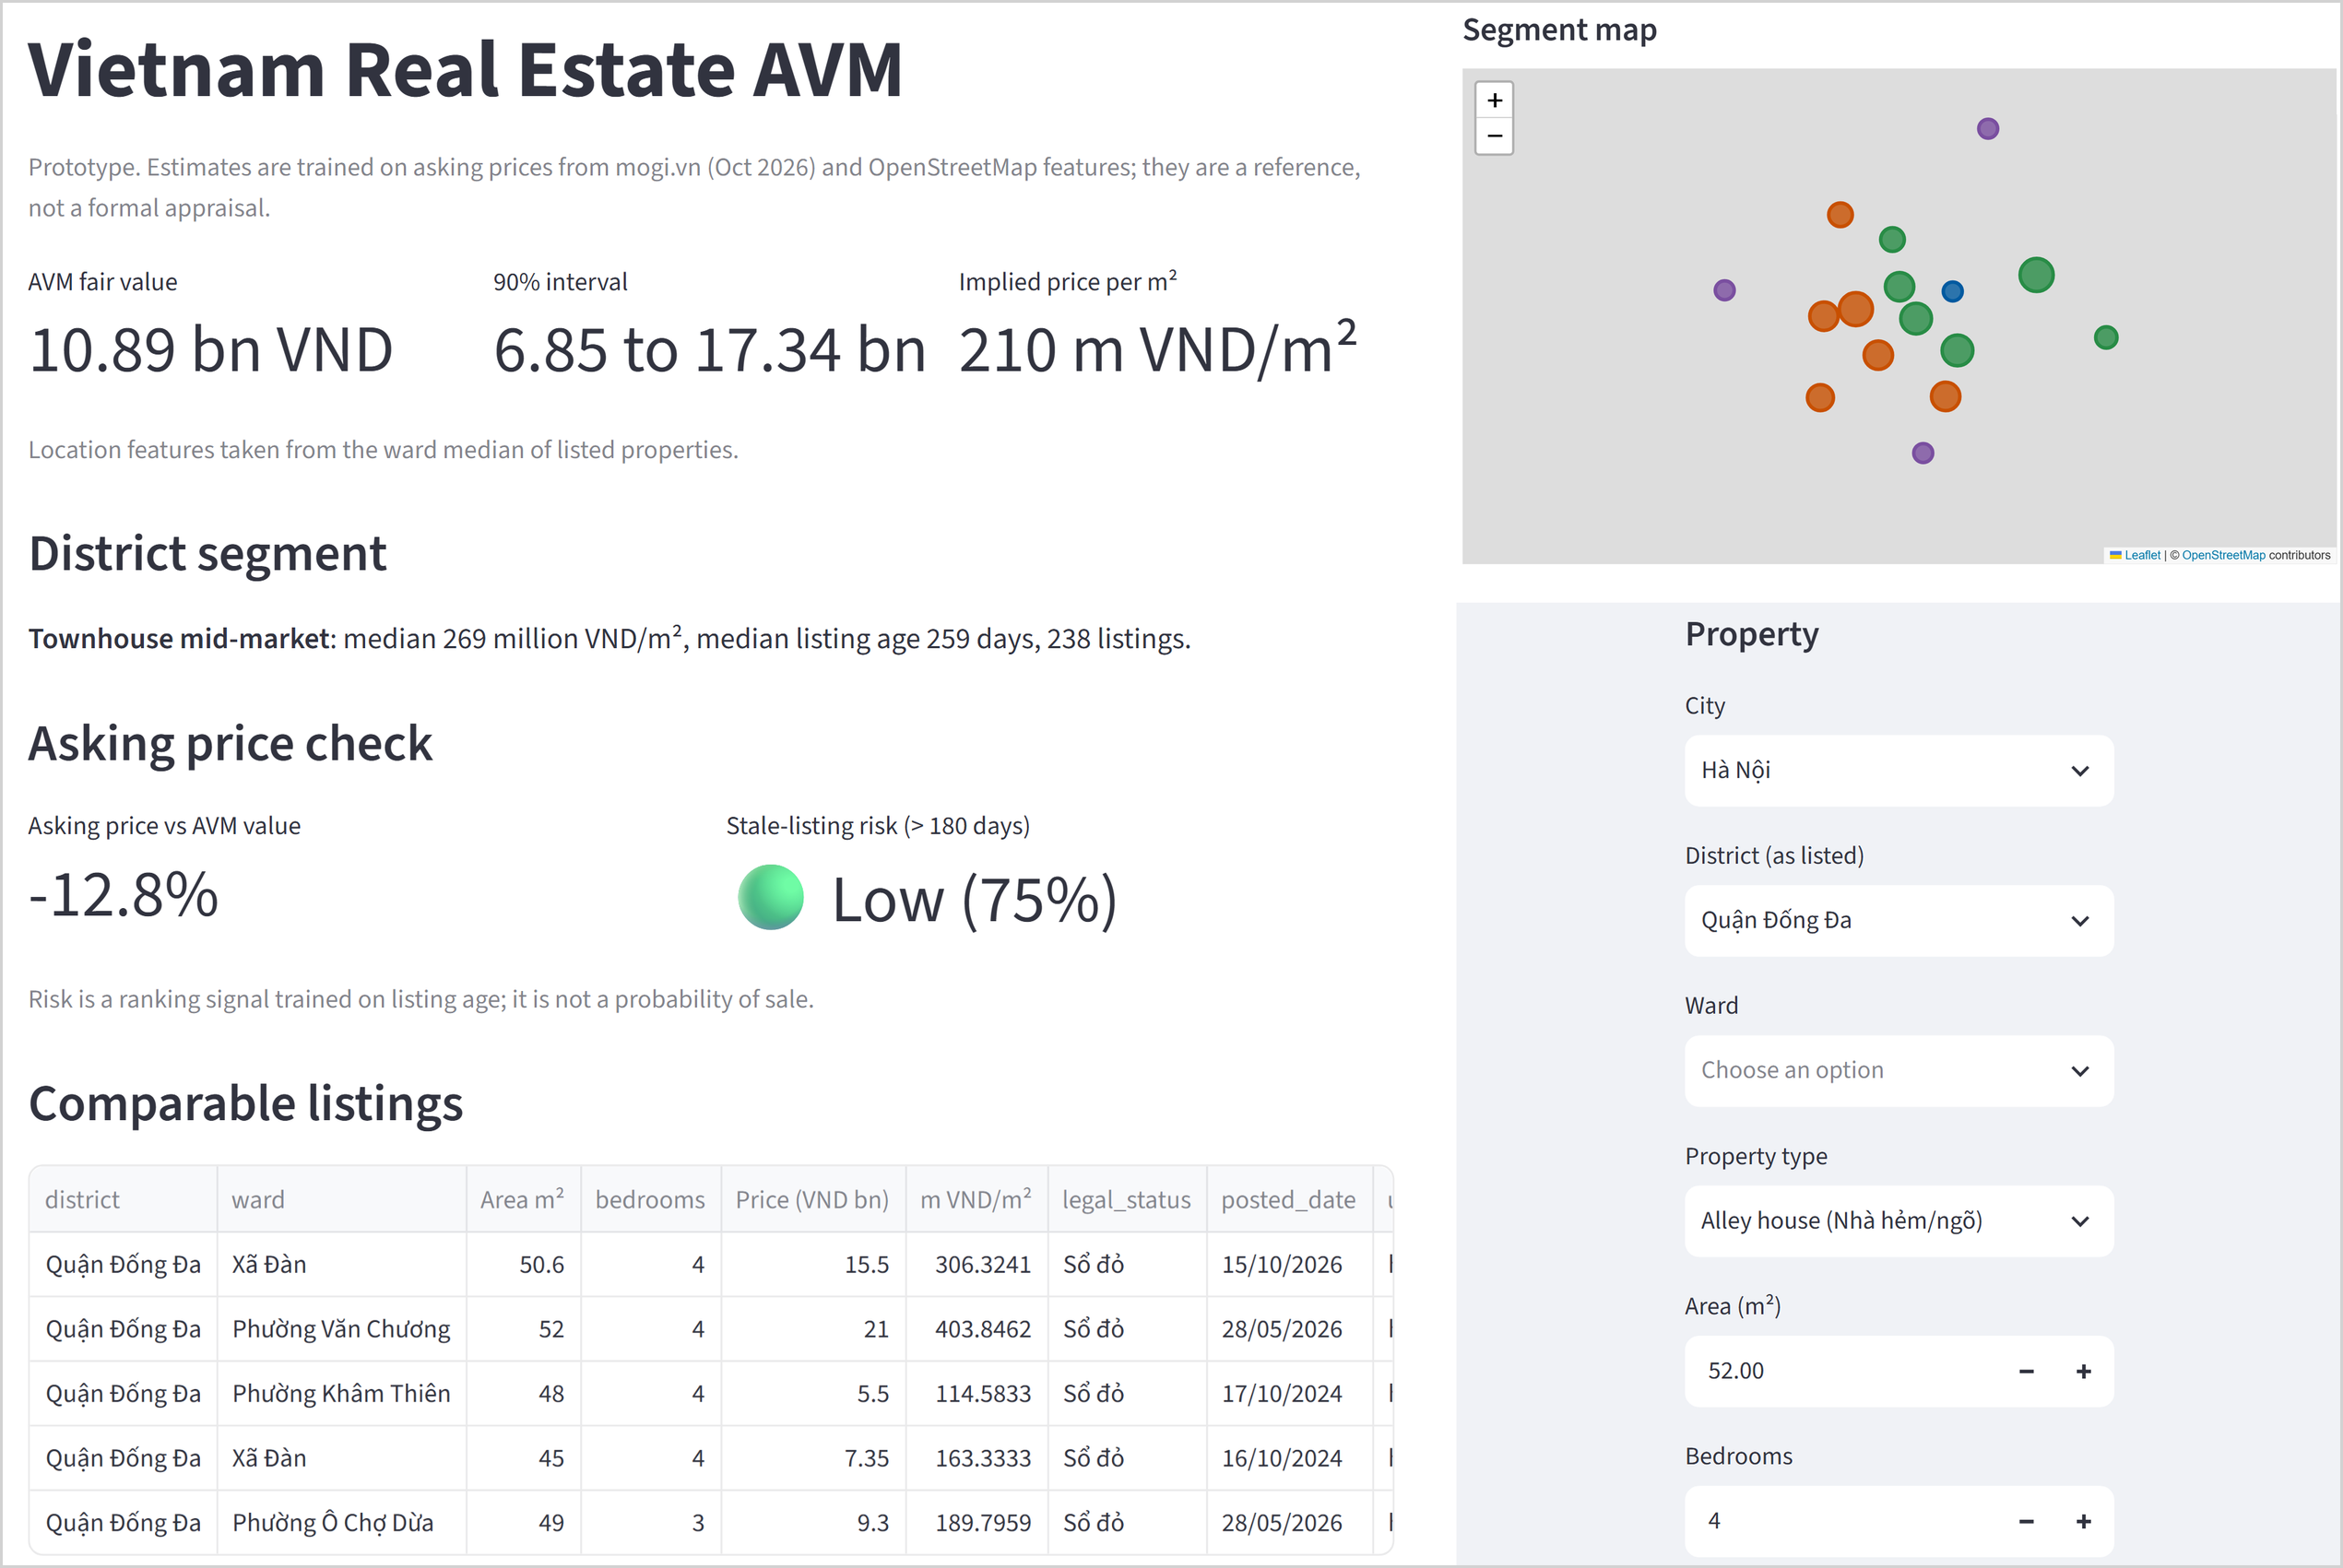
\includegraphics[width=0.85\textwidth]{dashboard_screenshot.png}};
\begin{scope}[x={(img.south east)}, y={(img.north west)}]
\foreach \n/\x/\y in {1/0.088/0.823, 2/0.193/0.527, 3/0.207/0.297, 4/0.717/0.981} {
  \node[circle, fill=accent, text=white, font=\sffamily\bfseries\scriptsize, inner sep=1.2pt, minimum size=11pt] at (\x,\y) {\n};}
\end{scope}
\end{tikzpicture}
\exsource{dashboard prototype with the engines trained on \srcmogi. Callouts: (1) fair value and 90\% range; (2) asking-price gap and stale-risk light; (3) five comparable listings; (4) district segment map. Inputs (right, below the map) are entered in the sidebar.}
\end{figure*}

\subsection{Executive management}
\textbf{Decision:} where to open offices, recruit brokers or commit capital. \textbf{Evidence:} Exhibit~\ref{fig:execmatrix} places every district by speed and price level. Districts to the left sell fastest; those in the upper left combine high prices with speed and deserve senior broker capacity. \textbf{KPI:} quarterly change in median listing age by segment.

\begin{table}[!t]
\caption{Each department owns one decision and uses at least two engines}
\label{tab:raci}
\tabsize
\begin{tabularx}{\columnwidth}{@{}>{\bfseries}Xccc@{}}
\toprule
Department & Fair value & Stale radar & Market Map \\
\midrule
Sales and brokerage & R & A, R & I \\
Marketing and research & C & I & A, R \\
Risk and credit & A, R & C & I \\
Executive management & I & I & A \\
Data team & R & R & R \\
\bottomrule
\end{tabularx}
\exsource{team design. R = responsible (uses daily), A = accountable (owns the decision), C = consulted, I = informed.}
\end{table}

\textbf{Every engine has a business owner (Exhibit~\ref{tab:raci}).} The data team runs all three engines. Each department owns the decision its engine feeds, which ties every model change to a business owner. 
% ---- inlined from sections/08_tools ----
\section{Tools and workflow}
\label{sec:tools}

\begin{table}[!htb]
\caption{Each layer uses a tool that scales, supports teamwork and needs no code from managers}
\label{tab:tools}
\tabsize
\begin{tabularx}{\columnwidth}{@{}>{\bfseries}p{1.6cm}p{1.9cm}X@{}}
\toprule
Layer & Tool & Why it fits \\
\midrule
Collection & Python & Resumes after interruptions; \throughput{} listings an hour with polite pacing \\
Map data & OpenStreetMap & Free, open licence; one download per city each quarter \\
Storage & Files now; cloud database later & No setup for the prototype; spatial queries and access control in production \\
Models & Regression, XGBoost, SHAP & A transparent baseline plus an accurate model, both explainable \\
Interface & Streamlit dashboard & A valuation in a browser, no code needed \\
Reporting & \LaTeX{} & Figures and numbers generated automatically from the analysis \\
Teamwork & Git & Shared history; one automated rebuild of data, models and reports \\
\bottomrule
\end{tabularx}
\exsource{team design.}
\end{table}

\textbf{Open-source tools keep the prototype cheap and the path to production short.} Each tool was chosen on three tests: does it scale to the full market, can a team work on it together, and can a manager use the output without code.

\textbf{The prototype runs on a laptop.} One automated pipeline collects the listings, adds the map data, re-trains the models and refreshes every exhibit. In production the same pipeline moves to a cloud database with spatial queries, runs weekly, and keeps every model version with its accuracy record. A standalone browser version of the dashboard accompanies this report.

\textbf{From data refresh to a manager's decision in four steps.} (1) The weekly collection and cleaning job updates the property table. (2) The engines re-score every listing, and re-train monthly if accuracy on new listings falls below the launch level. (3) The dashboard and the district brief refresh automatically. (4) A broker enters a home and an asking price and reads the fair value, its range, the gap, the stale-risk light and five comparables (Exhibit~\ref{fig:dashboard}).

\textbf{Governance keeps the numbers trustworthy.}
\begin{itemize}
\item \textbf{Change control.} A new model version goes live only after its business owner (Exhibit~\ref{tab:raci}) signs off its accuracy report by type.
\item \textbf{Monitoring.} A monthly report tracks accuracy by type, stale flags and broker usage.
\item \textbf{Access.} Brokers see estimates; only the data team sees raw listings; no personal data is stored.
\end{itemize}
Exhibit~\ref{tab:tools} lists the tool behind each layer and why it fits. 
% ---- inlined from sections/09_value ----
\section{Value and ROI}
\label{sec:value}

\begin{table}[!t]
\caption{Base case: partner value of VND \partnerBase{} bn a year leaves net value of \netPartnerBase{} bn, \roiBase{} times the run cost; the conservative case does not cover its cost}
\label{tab:value}
\scriptsize
% ---- inlined from tables/value_inputs.tex ----
\begin{tabularx}{\linewidth}{@{}Xrrr@{}}
\toprule
Input & Cons. & Base & Opt. \\
\midrule
Brokers using the tool & 100 & 300 & 500 \\
Valuations per broker a month & 10.0 & 20.0 & 25.0 \\
Hours saved per valuation & 0.50 & 1.00 & 1.25 \\
Broker cost (VND m/hour) & 0.10 & 0.15 & 0.20 \\
Mortgage files pre-screened a year & 1,000 & 3,000 & 6,000 \\
Estimates within ±10\% (PPE10)$^{*}$ & 30\% & 30\% & 30\% \\
PPE10 files where the bank waives appraisal & 30\% & 50\% & 70\% \\
Cost of an appraisal (VND m) & 1.50 & 2.50 & 4.00 \\
Run cost, 3-person team (VND m/year) & 3,000 & 2,200 & 1,600 \\
Buyer deals guided a year & 300 & 1,000 & 2,500 \\
Listings above the 90\% range$^{*}$ & 4\% & 4\% & 4\% \\
Median excess above the range$^{*}$ & 12\% & 12\% & 12\% \\
Share of excess negotiated away & 10\% & 20\% & 30\% \\
Median asking price (VND bn)$^{*}$ & 9.60 & 9.60 & 9.60 \\
\bottomrule
\end{tabularx} 

\vspace{3pt}
% ---- inlined from tables/value_results.tex ----
\begin{tabularx}{\linewidth}{@{}Xrrr@{}}
\toprule
Annual value, VND bn & Cons. & Base & Opt. \\
\midrule
Broker time saved & 0.6 & 10.8 & 37.5 \\
Bank appraisal cost avoided & 0.1 & 1.1 & 5.0 \\
Run cost & 3.0 & 2.2 & 1.6 \\
\textbf{Net partner value} & \textbf{$-$2.3} & \textbf{9.7} & \textbf{40.9} \\
\textbf{ROI (net value / run cost)} & \textbf{$-$0.8x} & \textbf{4.4x} & \textbf{25.6x} \\
Buyer overpayment avoided (not in ROI) & 1.6 & 10.4 & 39.0 \\
\bottomrule
\end{tabularx} 
\exsource{$^{*}$ measured in this analysis; all other inputs are team assumptions; ROI = (partner value $-$ run cost) / run cost.}
\end{table}


\begin{figure*}[t]
\caption{Broker adoption drives the business case more than any accuracy metric}
\label{fig:tornado}
\centering
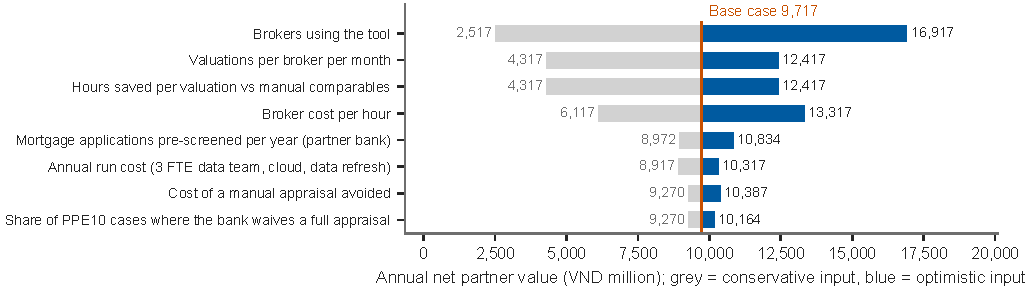
\includegraphics[width=0.9\textwidth]{value_tornado.pdf}
\exsource{team assumptions in Exhibit~\ref{tab:value}; each bar varies one input between its conservative and optimistic value, holding the others at base.}
\end{figure*}

\begin{figure*}[t]
\caption{Twelve months in three phases, with a go or no-go gate at the end of each phase}
\label{fig:roadmap}
\centering
\resizebox{0.95\textwidth}{!}{% ---- inlined from diagrams/roadmap.tex ----
% Implementation roadmap (Gantt style), months 1 to 12.
% Task names sit in a left column outside the timeline; bars start on the month grid; owners sit right of each bar;
% milestones sit on their own row below each phase.
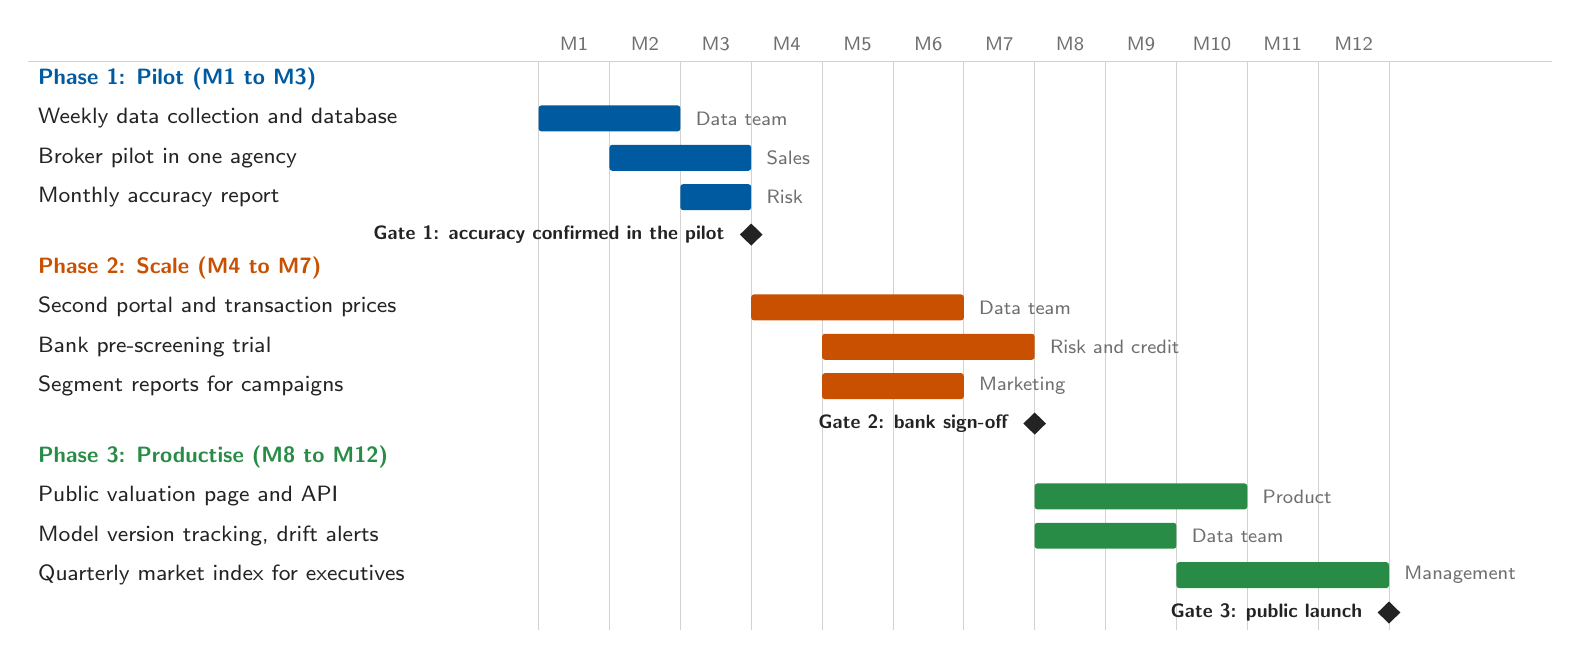
\begin{tikzpicture}[font=\sffamily\footnotesize, x=0.9cm, y=0.5cm]
\def\T{7.2}% x where month 1 starts
% month header and grid
\foreach \m in {1,...,12} { \node[text=medgray, font=\sffamily\scriptsize] at (\T+\m-0.5,0.9) {M\m}; }
\foreach \m in {0,...,12} { \draw[rulecolor, line width=0.3pt] (\T+\m,0.45) -- (\T+\m,-14.0); }
\draw[rulecolor, line width=0.5pt] (0,0.45) -- (\T+14.3,0.45);
% phase titles
\newcommand{\phase}[3]{\node[anchor=west, font=\sffamily\bfseries\footnotesize, text=#3] at (0,#1) {#2};}
\phase{0}{Phase 1: Pilot (M1 to M3)}{brand}
\phase{-4.8}{Phase 2: Scale (M4 to M7)}{accent}
\phase{-9.6}{Phase 3: Productise (M8 to M12)}{greenframe}
% task: y, name, start month (0-based), end month, colour, owner
\newcommand{\task}[6]{%
  \node[anchor=west, text=darkgray] at (0,#1) {#2};
  \fill[#5, rounded corners=1pt] (\T+#3,#1-0.33) rectangle (\T+#4,#1+0.33);
  \node[anchor=west, text=medgray, font=\sffamily\scriptsize] at (\T+#4+0.08,#1) {#6};}
\task{-1}{Weekly data collection and database}{0}{2}{brand}{Data team}
\task{-2}{Broker pilot in one agency}{1}{3}{brand}{Sales}
\task{-3}{Monthly accuracy report}{2}{3}{brand}{Risk}
\task{-5.8}{Second portal and transaction prices}{3}{6}{accent}{Data team}
\task{-6.8}{Bank pre-screening trial}{4}{7}{accent}{Risk and credit}
\task{-7.8}{Segment reports for campaigns}{4}{6}{accent}{Marketing}
\task{-10.6}{Public valuation page and API}{7}{10}{greenframe}{Product}
\task{-11.6}{Model version tracking, drift alerts}{7}{9}{greenframe}{Data team}
\task{-12.6}{Quarterly market index for executives}{9}{12}{greenframe}{Management}
% milestones: diamond on the month boundary, label to its left on a free row
\newcommand{\milestone}[3]{%
  \fill[darkgray] (\T+#1,#2+0.28) -- (\T+#1+0.16,#2) -- (\T+#1,#2-0.28) -- (\T+#1-0.16,#2) -- cycle;
  \node[anchor=east, text=darkgray, font=\sffamily\scriptsize\bfseries] at (\T+#1-0.24,#2) {#3};}
\milestone{3}{-3.95}{Gate 1: accuracy confirmed in the pilot}
\milestone{7}{-8.75}{Gate 2: bank sign-off}
\milestone{12}{-13.55}{Gate 3: public launch}
\end{tikzpicture} }
\exsource{team plan; owners refer to the departments in Section~\ref{sec:xf}.}
\end{figure*}

\textbf{The base case pays: net partner value of VND \netPartnerBase{} billion a year, \roiBase{} times the run cost.} Partners gain VND \partnerBase{} billion a year against a run cost of VND \runCostBase{} billion (Exhibit~\ref{tab:value}). The figures are scenario estimates on labelled assumptions, not measured outcomes. Three levers create the value:
\begin{itemize}
\item \textbf{Broker time saved:} an instant estimate and range replace a manual search for comparables.
\item \textbf{Bank appraisal cost avoided:} a partner bank waives part of the full appraisals where the estimate falls within ±10\% (\xgbPPEten{} of homes).
\item \textbf{Buyer overpayment avoided:} only listings above the 90\% range count (\shareAboveBand{} of listings, median excess \excessAboveBand), so model error is not counted. This value goes to buyers, outside the ROI.
\end{itemize}

\textbf{Adoption, not accuracy, decides the case (Exhibit~\ref{fig:tornado}).} With 100 brokers making 10 valuations a month and saving half an hour each, the platform loses VND \netPartnerConsAbs{} billion a year. The number of brokers using the tool moves net value more than any other input.

\textbf{The strategic value goes beyond money.} It would be the first public valuation of all property types in the two cities. The weekly listing panel becomes a price index and time-on-market record that competitors cannot copy quickly. 
% ---- inlined from sections/10_roadmap ----
\section{Roadmap, risks and recommendations}
\label{sec:roadmap}

\begin{table}[!t]
\caption{Five risks, each with a mitigation; the asking-price gap and the stale label matter most for the current results}
\label{tab:risks}
\scriptsize
\begin{tabularx}{\columnwidth}{@{}>{\bfseries\raggedright\arraybackslash}p{2.2cm}c>{\raggedright\arraybackslash}X@{}}
\toprule
Risk & L / I & Mitigation \\
\midrule
Listing site changes its pages or blocks collection & M / H & Tested page readers; adaptive pacing; second portal in Phase 2; negotiate a data feed \\
Asking prices differ from transaction prices & H / H & Calibrate on bank appraisals or notarised prices in Phase 2; present results as asking-price references until then \\
Stale label is noisy (refreshed dates, unseen sales) & H / M & Creation-date labels now; delisting events from weekly collection give a true time-to-sale label \\
Accuracy drifts as prices move & M / M & Monthly accuracy report by type; re-train when PPE20 falls 5 points below launch \\
Legal and reputational risk of publishing valuations & L / H & Ranges, not single numbers; disclaimers; no personal data; published method and accuracy \\
\bottomrule
\end{tabularx}
\exsource{team analysis. L / I = likelihood / impact: H high, M medium, L low.}
\end{table}

\textbf{Twelve months, three phases, each closed by a measured gate (Exhibit~\ref{fig:roadmap}).} Exhibit~\ref{tab:risks} lists the five risks and their mitigation.

\textbf{Each gate is a number the steering group can check.}
\begin{itemize}
\item \textbf{Gate 1, month 3 (continue to scale?).} On pilot deals, apartments and alley houses stay at or above the test hit rate of \ppeTwentyApartment{} within ±20\%. Pilot brokers use the tool weekly. If accuracy drops, the pilot runs one more quarter.
\item \textbf{Gate 2, month 7 (start lending use?).} The partner bank compares fair values with its own appraisals on live files and agrees a waiver rule for files within ±10\%. Active brokers reach the 300 target.
\item \textbf{Gate 3, month 12 (launch publicly?).} Accuracy by type is published and stable for three monthly reports in a row. Legal review of the disclaimers is complete.
\end{itemize}

\subsection{Recommendations}
\begin{enumerate}
\item \textbf{Launch the Fair Value Engine to brokers for apartments and alley houses first.} These types reach \ppeTwentyApartment{} and \ppeTwentyAlleyHouse{} within ±20\% on unseen homes. Show every estimate with its 90\% range and five comparables.
\item \textbf{Keep street-front houses, villas and land on desk review.} Their hit rates (\ppeTwentyStreetFrontHouse, \ppeTwentyVillaTerraced, \ppeTwentyLand) are too low for automated use. Add frontage quality, plot shape and business-use fields to the listing form.
\item \textbf{Sell the Stale Listing Radar as a priority list, not an overpricing detector.} Its top 10\% of listings are stale \topDecileLift{} times as often as average, which justifies a weekly review list. Base repricing advice on the price gap from the Fair Value Engine.
\item \textbf{Build a true time-to-sale label in Phase 1.} Weekly data collection shows when listings disappear. Within three months this replaces the creation-age proxy.
\item \textbf{Calibrate on transactions before any lending use.} Before the bank trial, re-measure accuracy against appraisal or notarised prices.
\item \textbf{Make broker adoption the first business KPI.} The case turns positive only with broad adoption. Target 300 active brokers by the end of Phase 2 and report usage next to accuracy every month.
\end{enumerate} 

{\footnotesize\setlength{\bibsep}{0.8pt}
\begin{thebibliography}{21}
\providecommand{\natexlab}[1]{#1}
\providecommand{\url}[1]{\texttt{#1}}
\expandafter\ifx\csname urlstyle\endcsname\relax
  \providecommand{\doi}[1]{doi: #1}\else
  \providecommand{\doi}{doi: \begingroup \urlstyle{rm}\Url}\fi

\bibitem[{Brands Vietnam}(2021)]{rever2021}
{Brands Vietnam}.
\newblock
  \href{https://www.brandsvietnam.com/21900-Rever-them-trieu-USD-rong-duong-cho-proptech}{{Rever
  thêm triệu USD, rộng đường cho proptech}}, 2021.

\bibitem[{Báo Pháp luật}(2022)]{onehousing_bpl2022}
{Báo Pháp luật}.
\newblock
  \href{https://baophapluat.vn/nhung-con-so-gay-soc-sau-1-thang-ra-mat-cua-cong-cu-dinh-gia-nha-onehousing-post451212.html}{{Những
  con số sau 1 tháng ra mắt của công cụ định giá nhà
  OneHousing}}, 2022.

\bibitem[Chen and Guestrin(2016)]{chen2016}
Tianqi Chen and Carlos Guestrin.
\newblock \href{https://doi.org/10.1145/2939672.2939785}{{XGBoost}: A Scalable
  Tree Boosting System}.
\newblock In \emph{Proceedings of the 22nd ACM SIGKDD International Conference
  on Knowledge Discovery and Data Mining}, pages 785--794, 2016.

\bibitem[Debrezion et~al.(2007)Debrezion, Pels, and Rietveld]{debrezion2007}
Ghebreegziabiher Debrezion, Eric Pels, and Piet Rietveld.
\newblock \href{https://doi.org/10.1007/s11146-007-9032-z}{The Impact of
  Railway Stations on Residential and Commercial Property Value: A
  Meta-analysis}.
\newblock \emph{Journal of Real Estate Finance and Economics}, 35:\penalty0
  161--180, 2007.

\bibitem[{e27}(2025)]{citics_e27_2025}
{e27}.
\newblock
  \href{https://e27.co/citics-lands-us2-1m-to-digitise-mortgage-lending-and-real-estate-transactions-20250515/}{Citics
  Lands {US\$2.1M} to Digitise Mortgage Lending and Real Estate Transactions},
  2025.

\bibitem[Gibbons and Machin(2005)]{gibbons2005}
Stephen Gibbons and Stephen Machin.
\newblock \href{https://doi.org/10.1016/j.jue.2004.10.002}{Valuing Rail Access
  Using Transport Innovations}.
\newblock \emph{Journal of Urban Economics}, 57:\penalty0 148--169, 2005.

\bibitem[{Inman}(2021)]{inman2021}
{Inman}.
\newblock
  \href{https://inman.com/2021/11/03/the-zestimate-comes-back-to-bite-reactions-to-the-end-of-zillow-offers}{The
  Zestimate Comes Back to Bite: Reactions to the End of Zillow Offers}, 2021.

\bibitem[{International Association of Assessing Officers}(2013)]{iaao2013}
{International Association of Assessing Officers}.
\newblock
  \href{https://www.iaao.org/media/standards/Standard_on_Ratio_Studies.pdf}{Standard
  on Ratio Studies}.
\newblock Technical report, IAAO, 2013.

\bibitem[{International Association of Assessing Officers}(2018)]{iaao2018}
{International Association of Assessing Officers}.
\newblock
  \href{https://www.iaao.org/wp-content/uploads/Standard_on_Automated_Valuation_Models.pdf}{Standard
  on Automated Valuation Models ({AVMs})}.
\newblock Technical report, IAAO, 2018.

\bibitem[Lei et~al.(2018)Lei, G'Sell, Rinaldo, Tibshirani, and
  Wasserman]{lei2018}
Jing Lei, Max G'Sell, Alessandro Rinaldo, Ryan~J. Tibshirani, and Larry
  Wasserman.
\newblock
  \href{https://doi.org/10.1080/01621459.2017.1307116}{Distribution-Free
  Predictive Inference for Regression}.
\newblock \emph{Journal of the American Statistical Association}, 113:\penalty0
  1094--1111, 2018.

\bibitem[Lundberg and Lee(2017)]{lundberg2017}
Scott~M. Lundberg and Su-In Lee.
\newblock A unified approach to interpreting model predictions.
\newblock In \emph{Advances in Neural Information Processing Systems 30 (NIPS
  2017)}, pages 4765--4774, 2017.

\bibitem[Malpezzi(2003)]{malpezzi2003}
Stephen Malpezzi.
\newblock \href{https://doi.org/10.1002/9780470690680.ch5}{Hedonic Pricing
  Models: A Selective and Applied Review}.
\newblock In \emph{Housing Economics and Public Policy}, pages 67--89.
  Blackwell Science, 2003.

\bibitem[Mayer et~al.(2019)Mayer, Bourassa, Hoesli, and
  Scognamiglio]{mayer2019}
Michael Mayer, Steven~C. Bourassa, Martin Hoesli, and Donato Scognamiglio.
\newblock \href{https://doi.org/10.1108/JERER-08-2018-0035}{Estimation and
  Updating Methods for Hedonic Valuation}.
\newblock \emph{Journal of European Real Estate Research}, 12:\penalty0
  134--150, 2019.

\bibitem[{PwC Vietnam}(2025)]{pwc2025}
{PwC Vietnam}.
\newblock
  \href{https://www.pwc.com/vn/en/publications/2025/vietnam-administrative-reform.pdf}{Vietnam
  Administrative Reform}, 2025.

\bibitem[Rosen(1974)]{rosen1974}
Sherwin Rosen.
\newblock \href{https://doi.org/10.1086/260169}{Hedonic Prices and Implicit
  Markets: Product Differentiation in Pure Competition}.
\newblock \emph{Journal of Political Economy}, 82:\penalty0 34--55, 1974.

\bibitem[Sirmans et~al.(2005)Sirmans, Macpherson, and Zietz]{sirmans2005}
G.~Stacy Sirmans, David~A. Macpherson, and Emily~N. Zietz.
\newblock \href{https://doi.org/10.1080/10835547.2005.12090154}{The Composition
  of Hedonic Pricing Models}.
\newblock \emph{Journal of Real Estate Literature}, 13:\penalty0 3--43, 2005.

\bibitem[{Techcombank}(2023)]{techcombank_avm}
{Techcombank}.
\newblock
  \href{https://techcombank.com/thong-tin/thong-bao/cong-cu-dinh-gia-bat-dong-san-tu-dong}{{Công
  cụ định giá bất động sản tự động}}, 2023.

\bibitem[{VietnamFinance}(2022)]{propzy2022}
{VietnamFinance}.
\newblock
  \href{https://vietnamfinance.vn/startup-bat-dong-san-viet-tung-duoc-soft-bank-rot-von-bat-ngo-dung-hoat-dong-d85823.html}{{Startup
  bất động sản Việt từng được SoftBank rót vốn bất ngờ
  dừng hoạt động}}, 2022.

\bibitem[{Việt Nam News}(2024)]{hcmcmetro2024}
{Việt Nam News}.
\newblock
  \href{https://vietnamnews.vn/society/1689480/historic-milestone-hcm-city-s-first-metro-line-launches-after-years-of-delay.html}{Historic
  Milestone: {HCM} City's First Metro Line Launches after Years of Delay},
  2024.

\bibitem[{VnEconomy}(2022)]{onehousing_vne2022}
{VnEconomy}.
\newblock
  \href{https://vneconomy.vn/onehousing-cong-cu-dinh-gia-nha-thuc-day-minh-bach-hoa-thi-truong-bat-dong-san.htm}{{OneHousing:
  Công cụ định giá nhà thúc đẩy minh bạch hóa thị trường
  bất động sản}}, 2022.

\bibitem[{Zillow}(2026)]{zillow_zestimate}
{Zillow}.
\newblock \href{https://www.zillow.com/zestimate/}{What Is a Zestimate?
  Zillow's Zestimate Accuracy}, 2026.

\end{thebibliography}
}

\onecolumn
\appendix
% ---- inlined from sections/appendix ----
\section*{Technical appendix}
\addcontentsline{toc}{section}{Technical appendix}
\renewcommand{\thesubsection}{A\arabic{subsection}}

\subsection{Design safeguards}
\label{app:safeguards}
\begin{enumerate}
\item \textbf{No listing age among the radar's inputs.} The stale label is defined by listing age, so age as an input would reveal the answer (target leakage). Listing age, posted, updated and photo dates, the listing ID and anything derived from them are excluded.
\item \textbf{Price gap estimated on unseen listings.} The gap between asking price and fair value used by the radar comes from five-fold cross-validated predictions for training rows (out-of-fold) and from the held-out model for test rows. An in-sample gap would carry the training fit into the classifier.
\item \textbf{Listing age from creation, not from the posted date.} The site assigns listing IDs in creation order. IDs are only weakly related to posted dates (Spearman $\rho = \rhoIDposted$) but track first photo-upload dates almost exactly ($\rho = \rhoIDphoto$). Also, \shareRefreshed{} of listings show a posted date more than 30 days after their photos were uploaded. The label therefore uses the creation date implied by the listing ID, calibrated to photo dates with an isotonic fit. The median listing age is \medAgePosted{} days from the posted date, \medAgeCreated{} days from the first photo and \medAgeID{} days from the listing ID.
\item \textbf{No poster account age among the radar's inputs.} An account cannot post before it exists, so account age bounds listing age mechanically; it is excluded for the same reason as item 1.
\end{enumerate}
The accessibility index is the first principal component of six inverted distances (metro, school, hospital, park, market, centre); it explains \accVar{} of their variance, with loadings between \accMinLoad{} and \accMaxLoad.

\subsection{Accuracy by city and type}
\label{app:metrics}
The gradient-boosting model has a median absolute error of \xgbMdAPE, PPE10 of \xgbPPEten{} and a coefficient of dispersion of \xgbCOD. Its price-related differential of \xgbPRD{} lies above the 0.98 to 1.03 range used in ratio studies \citep{iaao2013}. Split-conformal intervals calibrated on out-of-fold errors by type cover \confCovType{} of test homes (Exhibit~\ref{tab:segmetrics}).

\begin{table}[H]
\caption{Gradient boosting beats the regression in most city and type cells; land and street-front houses carry the widest errors}
\label{tab:segmetrics}
\centering\tabsize
% ---- inlined from tables/avm_metrics_by_segment.tex ----
\begin{tabular}{llrrrrrrrr}
\toprule
City & Type & N & \multicolumn{2}{c}{RMSE (log)} & \multicolumn{2}{c}{PPE20} & \multicolumn{2}{c}{MdAPE} & COD \\
 & & & OLS & XGB & OLS & XGB & OLS & XGB & XGB \\
\midrule
Hanoi & Villa / terraced & 55 & 0.343 & 0.292 & 47\% & 49\% & 21.3\% & 21.1\% & 23.0 \\
Hanoi & Apartment & 126 & 0.312 & 0.243 & 50\% & 59\% & 19.9\% & 16.8\% & 20.2 \\
Hanoi & Alley house & 156 & 0.340 & 0.307 & 46\% & 55\% & 21.4\% & 18.6\% & 22.8 \\
Hanoi & Street-front house & 100 & 0.527 & 0.431 & 22\% & 38\% & 38.7\% & 27.6\% & 36.2 \\
Hanoi & Land & 90 & 0.537 & 0.564 & 38\% & 37\% & 26.9\% & 27.7\% & 47.0 \\
HCMC & Villa / terraced & 63 & 0.423 & 0.339 & 48\% & 46\% & 22.6\% & 23.0\% & 26.7 \\
HCMC & Apartment & 149 & 0.399 & 0.344 & 49\% & 62\% & 20.4\% & 15.1\% & 26.9 \\
HCMC & Alley house & 144 & 0.309 & 0.234 & 60\% & 73\% & 15.6\% & 12.6\% & 16.5 \\
HCMC & Street-front house & 86 & 0.443 & 0.330 & 31\% & 48\% & 34.0\% & 21.8\% & 26.7 \\
HCMC & Land & 85 & 0.593 & 0.435 & 41\% & 51\% & 24.6\% & 16.4\% & 33.7 \\
\bottomrule
\end{tabular} 
\exsource{\srcmogi; \Ntest{} held-out test homes.}
\end{table}

\subsection{Stale Listing Radar and Market Map checks}
\label{app:robust}
Exhibit~\ref{tab:stalecomp} compares the radar with a price-gap rule and a logistic regression on the test set. With the posted-date label the AUC is near 1, because that label mainly records whether a broker account keeps re-posting the listing (Exhibit~\ref{tab:robust}). This is why the creation-date label is preferred. \textbf{Market Map.} Silhouette scores are low at every $k$; within the preferred range of 3 to 5 segments, $k = \kBest$ scores best (\silBest, against a target of 0.45). Ward hierarchical clustering with the same $k$ agrees with K-Means at an adjusted Rand index of \ariWard. Features are standardised and winsorised at ±2.5 standard deviations; listing age enters as a log median.

\begin{table}[H]
\caption{XGBoost ranks stale listings best; the price-gap rule is no better than chance}
\label{tab:stalecomp}
\centering\tabsize
% ---- inlined from tables/stale_comparison.tex ----
\begin{tabular}{lrrrrrr}
\toprule
Model & AUC & 95\% CI & PR-AUC & Brier & Top-decile precision & Top-decile capture \\
\midrule
Rule: AVM gap $>$ +15\% & 0.45 & 0.41 to 0.49 & 0.63 & -- & 57\% & 9\% \\
Logistic regression & 0.74 & 0.71 to 0.77 & 0.82 & 0.189 & 87\% & 13\% \\
XGBoost & 0.81 & 0.78 to 0.83 & 0.88 & 0.176 & 99\% & 15\% \\
\midrule
\multicolumn{7}{l}{Base rate (share stale in the test set): 65\%; N test = 1,054} \\
\bottomrule
\end{tabular} 
\exsource{\srcmogi; test set; label: on site more than \staleDays{} days since creation; Brier = mean squared error of the predicted probability.}
\end{table}

\begin{table}[H]
\caption{Ranking quality holds across creation-age thresholds; the posted-date label is predictable for the wrong reason}
\label{tab:robust}
\centering\tabsize
% ---- inlined from tables/stale_robustness.tex ----
\begin{tabular}{lrlrrr}
\toprule
Age measure & Days & Model & Positive share & AUC & 95\% CI \\
\midrule
Creation age (listing ID) & 180 & Rule (AVM gap $>$ 15\%) & 65\% & 0.45 & 0.41 to 0.49 \\
 &  & Logistic regression & 65\% & 0.74 & 0.71 to 0.77 \\
 &  & XGBoost & 65\% & 0.81 & 0.78 to 0.83 \\
\addlinespace[2pt]
Creation age (listing ID) & 60 & Rule (AVM gap $>$ 15\%) & 89\% & 0.51 & 0.46 to 0.57 \\
 &  & Logistic regression & 89\% & 0.83 & 0.80 to 0.86 \\
 &  & XGBoost & 89\% & 0.88 & 0.84 to 0.91 \\
\addlinespace[2pt]
Creation age (listing ID) & 90 & Rule (AVM gap $>$ 15\%) & 82\% & 0.46 & 0.42 to 0.50 \\
 &  & Logistic regression & 82\% & 0.82 & 0.79 to 0.85 \\
 &  & XGBoost & 82\% & 0.85 & 0.82 to 0.88 \\
\addlinespace[2pt]
Creation age (listing ID) & 120 & Rule (AVM gap $>$ 15\%) & 77\% & 0.46 & 0.42 to 0.50 \\
 &  & Logistic regression & 77\% & 0.81 & 0.78 to 0.85 \\
 &  & XGBoost & 77\% & 0.85 & 0.82 to 0.88 \\
\addlinespace[2pt]
Posted date (refreshed) & 60 & Rule (AVM gap $>$ 15\%) & 55\% & 0.47 & 0.44 to 0.51 \\
 &  & Logistic regression & 55\% & 0.96 & 0.95 to 0.98 \\
 &  & XGBoost & 55\% & 0.99 & 0.98 to 0.99 \\
\addlinespace[2pt]
Posted date (refreshed) & 90 & Rule (AVM gap $>$ 15\%) & 50\% & 0.48 & 0.45 to 0.52 \\
 &  & Logistic regression & 50\% & 0.91 & 0.90 to 0.93 \\
 &  & XGBoost & 50\% & 0.96 & 0.95 to 0.97 \\
\bottomrule
\end{tabular} 
\exsource{\srcmogi; held-out test sets; 95\% intervals from 1,000 (main) or 200 (robustness) bootstrap resamples.}
\end{table}

\subsection{Full regression table, model settings and data dictionary}
\label{app:ladder}
Exhibit~\ref{tab:ladderfull} gives the full regression ladder behind Exhibit~\ref{tab:ladder}. Exhibit~\ref{tab:hyper} lists the gradient-boosting settings, and Exhibit~\ref{tab:dict} the fields the engines use.

\begin{table}[H]
\caption{Hedonic regression ladder on log asking price}
\label{tab:ladderfull}
\centering\tabsize
% ---- inlined from tables/hedonic_ladder.tex ----
\begin{tabular}{lcccc}
\toprule
 & \textbf{(1)} & \textbf{(2)} & \textbf{(3)} & \textbf{(4)} \\
 & Physical & + District FE & + OSM spatial & + Interactions \\
\midrule
Log area & $0.931^{***}$ & $0.935^{***}$ & $0.929^{***}$ & $0.954^{***}$ \\
 & \footnotesize(0.046) & \footnotesize(0.025) & \footnotesize(0.025) & \footnotesize(0.057) \\[-1pt]
Bedrooms & $0.016$ & $-0.007$ & $-0.011$ & $-0.017^{**}$ \\
 & \footnotesize(0.012) & \footnotesize(0.008) & \footnotesize(0.008) & \footnotesize(0.008) \\[-1pt]
Bathrooms & $-0.002$ & $0.018^{*}$ & $0.022^{**}$ & $0.025^{***}$ \\
 & \footnotesize(0.013) & \footnotesize(0.010) & \footnotesize(0.010) & \footnotesize(0.009) \\[-1pt]
Storeys & $0.077^{***}$ & $0.064^{***}$ & $0.065^{***}$ & $0.066^{***}$ \\
 & \footnotesize(0.013) & \footnotesize(0.010) & \footnotesize(0.010) & \footnotesize(0.008) \\[-1pt]
Frontage (m) & $0.010$ & $0.005$ & $0.004$ & $0.006^{*}$ \\
 & \footnotesize(0.007) & \footnotesize(0.004) & \footnotesize(0.004) & \footnotesize(0.004) \\[-1pt]
Access road width (m) & $0.016^{***}$ & $0.013^{***}$ & $0.012^{***}$ & $0.013^{***}$ \\
 & \footnotesize(0.005) & \footnotesize(0.004) & \footnotesize(0.004) & \footnotesize(0.004) \\[-1pt]
Legal: sale contract & $0.146$ & $0.143^{*}$ & $0.144^{*}$ & $0.151^{**}$ \\
 & \footnotesize(0.091) & \footnotesize(0.086) & \footnotesize(0.078) & \footnotesize(0.076) \\[-1pt]
Legal: other/unknown & $0.067$ & $-0.090^{**}$ & $-0.097^{***}$ & $-0.109^{***}$ \\
 & \footnotesize(0.064) & \footnotesize(0.039) & \footnotesize(0.035) & \footnotesize(0.042) \\[-1pt]
Log distance to CBD &  &  & $-0.053$ & $-0.047$ \\
 &  &  & \footnotesize(0.052) & \footnotesize(0.053) \\[-1pt]
Log distance to metro &  &  & $-0.026$ & $-0.032$ \\
 &  &  & \footnotesize(0.035) & \footnotesize(0.032) \\[-1pt]
Log distance to school &  &  & $-0.009$ & $-0.006$ \\
 &  &  & \footnotesize(0.024) & \footnotesize(0.024) \\[-1pt]
Log distance to hospital &  &  & $-0.034$ & $-0.028$ \\
 &  &  & \footnotesize(0.028) & \footnotesize(0.024) \\[-1pt]
Log distance to park &  &  & $-0.054^{**}$ & $-0.055^{**}$ \\
 &  &  & \footnotesize(0.022) & \footnotesize(0.023) \\[-1pt]
Log distance to market/mall &  &  & $-0.059^{**}$ & $-0.055^{**}$ \\
 &  &  & \footnotesize(0.025) & \footnotesize(0.026) \\[-1pt]
Log distance to lake/river &  &  & $-0.015$ & $-0.012$ \\
 &  &  & \footnotesize(0.023) & \footnotesize(0.023) \\[-1pt]
Bus stops within 500 m &  &  & $-0.004$ & $-0.004$ \\
 &  &  & \footnotesize(0.004) & \footnotesize(0.003) \\[-1pt]
\midrule
District fixed effects & No & Yes & Yes & Yes \\
Type $\times$ city, type $\times$ log area & No & No & No & Yes \\
N & 5,268 & 5,268 & 5,268 & 5,268 \\
R$^2$ & 0.714 & 0.844 & 0.848 & 0.850 \\
Adjusted R$^2$ & 0.713 & 0.842 & 0.846 & 0.848 \\
5-fold CV RMSE (log) & 0.560 & 0.422 & 0.417 & 0.414 \\
\bottomrule
\end{tabular} 
\exsource{\srcmogi; \srcosm. Standard errors clustered by district in parentheses; $^{*}$, $^{**}$, $^{***}$: $p<0.10$, $0.05$, $0.01$. All columns include type and city dummies and missing-value flags; reference legal status: red or pink book (sổ đỏ/sổ hồng). Without district effects, physical and map features give R$^2$ = \RtwoE{} and CV RMSE = \cvE. CBD distance is not statistically different from zero within districts ($p = \pCbdC$); sale-contract listings ask more ($p = \pContractD$).}
\end{table}

\begin{table}[H]
\caption{Gradient-boosting settings, tuned by cross-validation on the training set only}
\label{tab:hyper}
\centering\tabsize
% ---- inlined from tables/hyperparams.tex ----
\begin{tabular}{lrr}
\toprule
Setting & Fair Value Engine & Stale Listing Radar \\
\midrule
Tree depth & 5 & 6 \\
Number of trees & 2,284 & 1,115 \\
Learning rate & 0.02 & 0.02 \\
Share of rows per tree & 0.79 & 0.88 \\
Share of features per tree & 0.54 & 0.67 \\
Minimum leaf size & 4.00 & 1.00 \\
Shrinkage penalty & 1.24 & 0.57 \\
Weight on stale listings & none & 0.53 \\
Search & 40 settings, 5-fold & 30 settings, 5-fold \\
\bottomrule
\end{tabular} 
\exsource{team analysis.}
\end{table}

\begin{table}[H]
\caption{Data dictionary: the fields the engines use}
\label{tab:dict}
{\tabsize% ---- inlined from tables/data_dictionary.tex ----
\begin{tabularx}{\textwidth}{@{}>{\bfseries}p{3.2cm}Xp{1.8cm}r@{}}
\toprule
Field & Description & Source & \% missing \\
\midrule
Asking price & Total asking price in VND (what the Fair Value Engine predicts) & Listing & 0 \\
Property type & Apartment, alley house, street-front house, villa or terraced, land & Listing & 0 \\
City, district, ward & Location as listed on the site (pre-2025 district names) & Listing & 0 \\
Map point & Latitude and longitude from the listing map & Listing & 0 \\
Area & Floor area (apartments) or land area (houses, villas, land), m$^2$ & Listing & 0 \\
Bedrooms, bathrooms & Room counts & Listing & 0 \\
Storeys & Number of floors, often read from the description & Listing text & 54 \\
Frontage & Plot width facing the street or alley, m & Listing & 29 \\
Plot depth & Plot depth, m & Listing & 31 \\
Access road width & Width of the alley or street in front, m & Listing text & 87 \\
Legal status & Red or pink book, sale contract, other or unknown & Listing & 0 \\
Text flags & Car access, corner lot, business use, lake view, near school, furnished, owner selling, urgent sale & Listing text & 0 \\
Seller profile & Registered broker profile or private account & Listing & 0 \\
Photos, description length & Number of photos; length of the description & Listing & 0 \\
Listing age & Days on the site since creation (label of the Stale Listing Radar only) & Derived & 0 \\
Distances & Distance to the centre, nearest metro station, school, hospital, park, market, water & Map data & 0 \\
Counts nearby & Bus stops, schools and other points within 500 m and 1 km & Map data & 0 \\
Accessibility index & One score combining six distances (higher = closer to amenities) & Map data & 0 \\
\bottomrule
\end{tabularx} }
\exsource{\srcmogi; \srcosm. Percent missing is measured before imputation.}
\end{table} 

\end{document}
